\documentclass[10pt]{article}
\usepackage[french]{babel}
\usepackage[utf8]{inputenc}
\usepackage[T1]{fontenc}
\usepackage{graphicx}
\usepackage[export]{adjustbox}
\graphicspath{ {./images/} }
\usepackage{caption}
\usepackage{amsmath}
\usepackage{amsfonts}
\usepackage{amssymb}
\usepackage[version=4]{mhchem}
\usepackage{stmaryrd}

\begin{document}
\captionsetup{singlelinecheck=false}
\section*{Réglage d'un pilote automatique pour un avion léger biplace}
\begin{figure}[h]
\begin{center}
  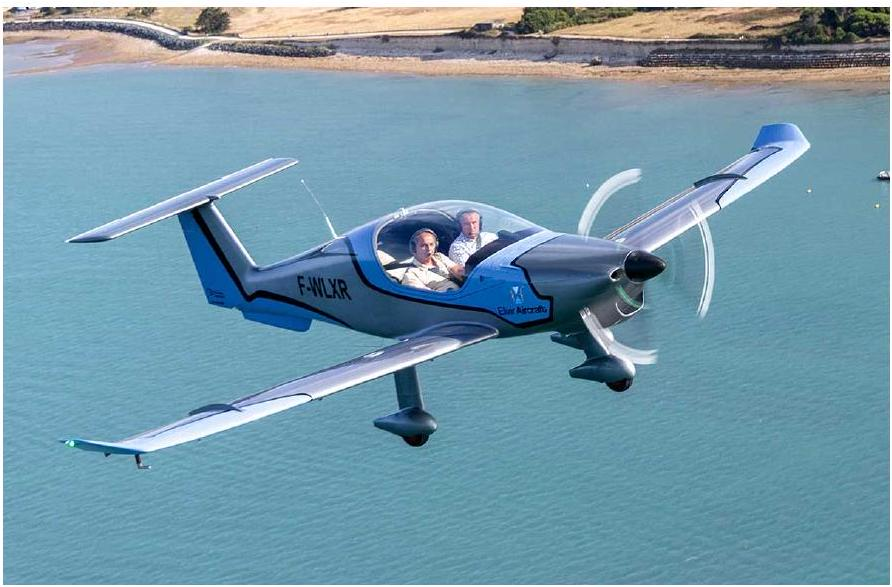
\includegraphics[alt={},max width=\textwidth]{b437a5a5-8562-4c88-96c5-adc15de36bac-01_587_892_719_587}
\captionsetup{labelformat=empty}
\caption{Figure 1 - L'Elixir en vol © Elixir Aircraft}
\end{center}
\end{figure}

\section*{Contexte}
L'entreprise française Elixir Aircraft commercialise un petit avion léger biplace, l'Elixir, destiné entre autres à la formation des pilotes (figure 1).\\
Cet avion est conçu selon une structure en OneShot, technique consistant à concevoir et fabriquer les éléments complexes (aile et fuselage) en une seule pièce en exploitant les avantages des matériaux composites, supprimant par la même occasion les difficultés causées par les assemblages. Les bénéfices sont nombreux : moins de pièces et moins d'assemblages se traduisent par un nombre de défaillances plus faible, la diminution de la maintenance et donc un coût réduit. Parallèlement, la sécurité est renforcée par la simplicité de la structure et les performances sont améliorées par la masse réduite. L'Elixir est ainsi 50 \% plus économe en carburant que la grande majorité des avions équivalents.

Un pilote automatique est un système permettant d'assurer un nombre important de fonctions, sans l'intervention du pilote, comme la stabilisation de l'avion, le suivi d'une trajectoire, le maintien à une altitude fixée ou même l'atterrissage. De nombreux avions sont équipés de tels types de systèmes.

L'Elixir est équipé d'un pilote automatique deux axes, permettant le contrôle du roulis et du tangage, respectivement via les ailerons et la gouverne de profondeur. Les différents constituants de l'avion sont présentés dans l'annexe A.\\
$\_\_\_\_$ Objectif\\
Objectif $\_\_\_\_$\\
Étudier la structure partielle de commande du pilote automatique et concevoir les lois de commande associées en vue de permettre la stabilisation en vol de croisière de façon à maintenir une altitude et une vitesse constantes.

\section*{Constitution du système de pilotage automatique}
L'implantation du pilote automatique fait appel en particulier à deux servomoteurs GSA 28 Smart Autopilot Servo agissant par le biais d'un système de transmission (par tringlerie) sur les ailerons d'une part, sur la gouverne de profondeur d'autre part. Les servomoteurs sont commandés par l'intermédiaire d'une unité GARMIN G3X Touch 10"

GDU460. Les commandes sont élaborées d'un point de vue plus général à partir des mesures de l'altitude, de l'orientation de l'avion et de la vitesse obtenues par un ensemble de capteurs. Les grandeurs acquises sont transmises à une unité ADAHRS (Air Data Attitude Heading Reference System) dont la fonction est de rendre les données exploitables par l'unité de traitement GARMIN GDU460.

Pour cette étude, restreinte au pilotage des seules vitesses horizontale et verticale, la structure du pilote automatique est représentée sur la figure 2 selon une architecture de régulation dite monovariable :

\begin{itemize}
  \item[-] la vitesse horizontale $V_{x}$ est pilotée par la force de propulsion $F_{m}$ du moteur thermique et de son hélice. Celle-ci est déterminée par un correcteur opérant à partir de l'écart de vitesse horizontale $\varepsilon_{x}$;
  \item[-] la vitesse verticale $V_{z}$ est pilotée par l'angle $\beta$ de la gouverne de profondeur, actionné par l'un des deux servomoteurs, à partir de l'écart de vitesse verticale $\varepsilon_{z}$.
\end{itemize}

\begin{figure}[h]
\begin{center}
  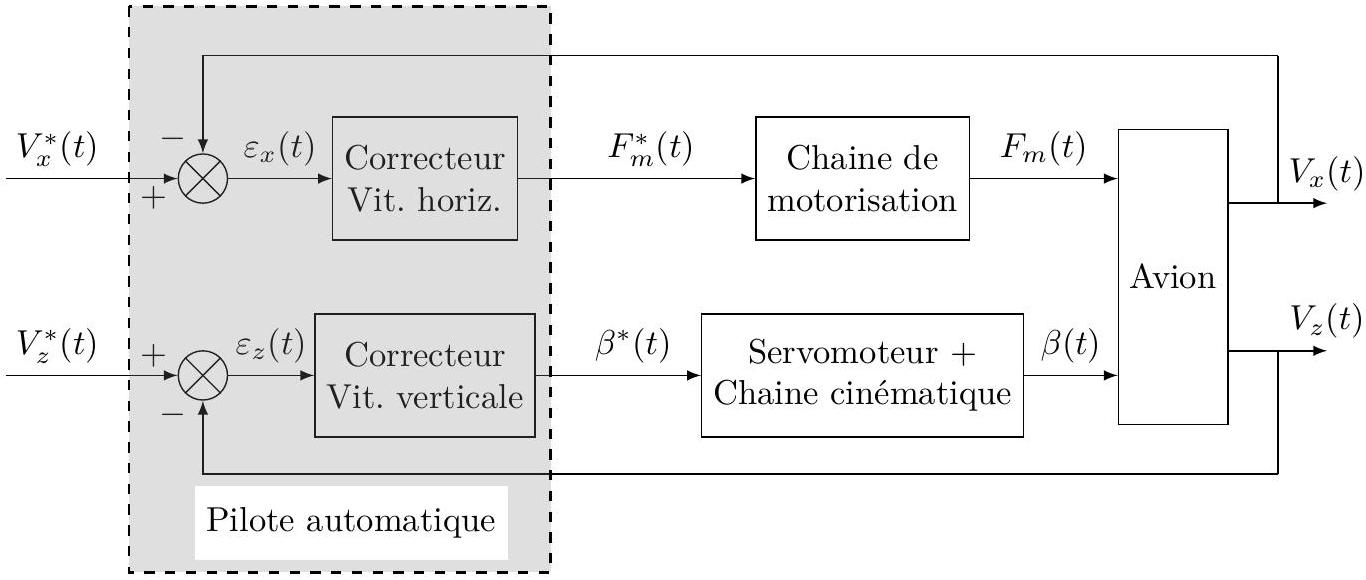
\includegraphics[alt={},max width=\textwidth]{b437a5a5-8562-4c88-96c5-adc15de36bac-02_580_1366_662_337}
\captionsetup{labelformat=empty}
\caption{Figure 2 - Structure restreinte du pilote automatique}
\end{center}
\end{figure}

Cette structure de régulation est dite monovariable car elle ne fait pas intervenir de terme de couplage de la vitesse verticale $V_{z}$ dans le calcul de la force de propulsion $F_{m}$ ni de la vitesse horizontale $V_{x}$ dans le calcul de l'angle de gouverne $\beta$. En pratique, les grandeurs de commande issues des correcteurs sont les consignes $F_{m}^{*}$ et $\beta^{*}$, respectivement de la force de propulsion $F_{m}$ générée par le moteur thermique et de l'angle de la gouverne de profondeur $\beta$.

\section*{Problématique et démarche de l'étude}
L'objectif de cette étude est le calcul des correcteurs des deux boucles de vitesse de façon à ce que le pilote automatique assure les contraintes du cahier des charges décrites par le diagramme d'exigences donné figure 3.

Pour atteindre cet objectif, la procédure de synthèse des lois de commande suit les phases suivantes :

\begin{itemize}
  \item[-] conception d'un modèle dynamique non linéaire qui doit permettre
  \begin{itemize}
    \item[-] la validation en simulation des performances du pilote automatique, au regard des exigences du cahier des charges,
    \item[-] la définition des modèles linéaires (par linéarisation au $1{ }^{\text {er }}$ ordre) pour le calcul des correcteurs des deux boucles d'asservissement ;
  \end{itemize}
  \item[-] calcul des paramètres des correcteurs du pilote automatique ;
  \item[-] analyse de la robustesse (capacité à conserver les performances souhaitées) du pilote automatique au regard de la variation de la masse volumique de l'air en fonction de l'altitude.
\end{itemize}

Cette dernière phase fera également l'objet d'une synthèse globale et l'ensemble sera complété par une étude intermédiaire en vue de définir le modèle de la chaine cinématique de la gouverne de profondeur.

\section*{Partie A - Comportement dynamique de l'avion}
$\_\_\_\_$ Objectif $\_\_\_\_$\\
Déterminer un modèle dynamique décrivant l'évolution de l'altitude de l'avion en prenant l'angle de la gouverne de profondeur et la force exercée par le moteur thermique et son hélice comme entrées de commande, la force exercée par le vent comme entrée de perturbation.

\begin{figure}[h]
\begin{center}
  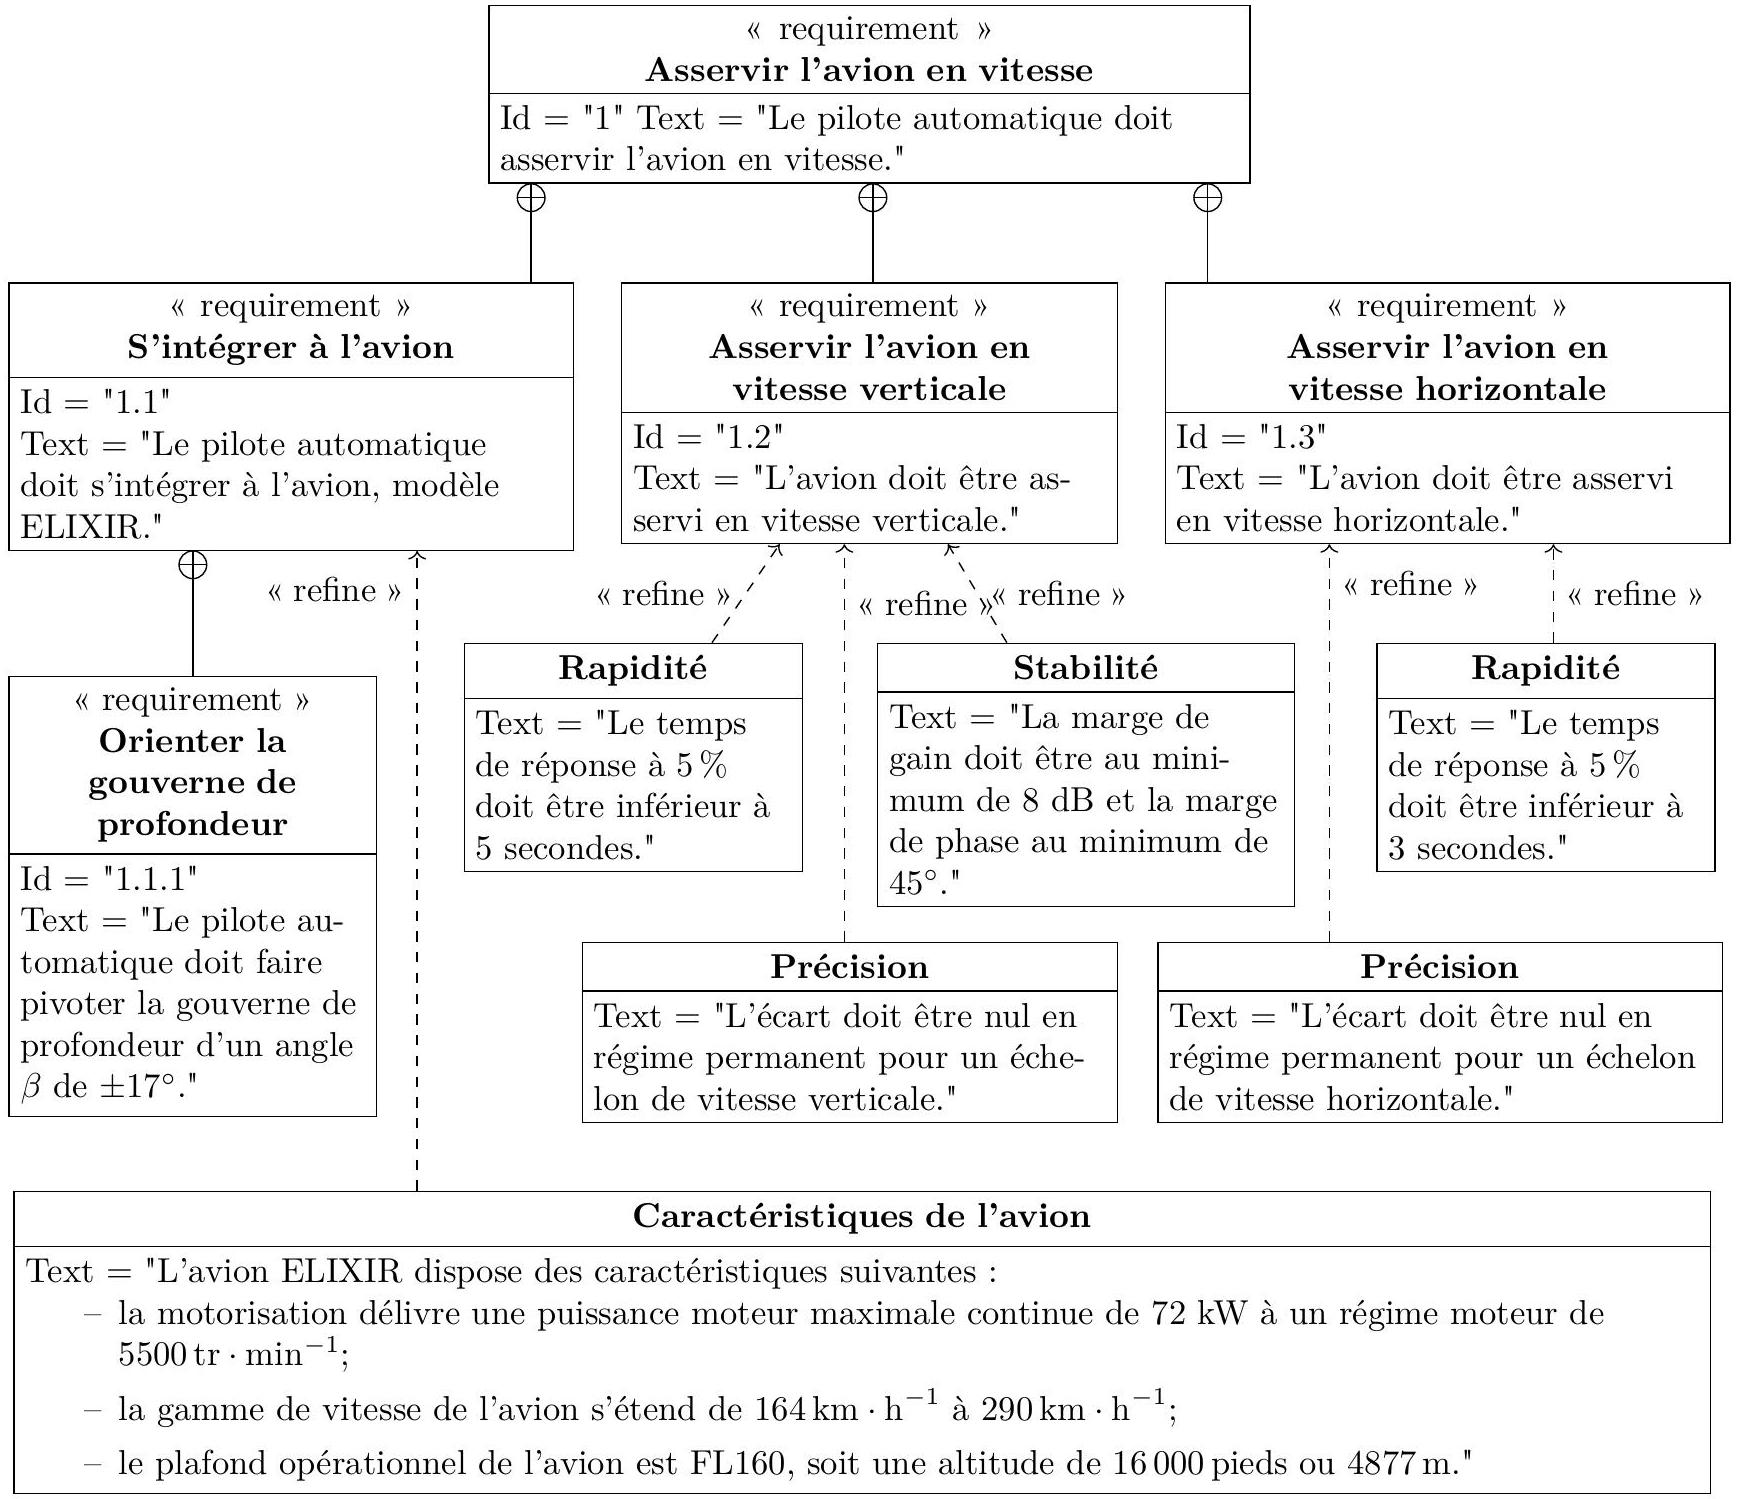
\includegraphics[alt={},max width=\textwidth]{b437a5a5-8562-4c88-96c5-adc15de36bac-03_1499_1737_123_164}
\captionsetup{labelformat=empty}
\caption{Figure 3 - Diagramme d'exigences pour l'asservissement de vitesse}
\end{center}
\end{figure}

\section*{Repères et paramétrage associés à l'avion}
On définit (voir figure 4) les points $G$ et $B$, respectivement centre de gravité de l'avion et centre de poussée de la gouverne de profondeur, et les repères suivants.

\begin{itemize}
  \item[-] $R_{0}=\left(O, \vec{x}_{0}, \vec{y}_{0}, \vec{z}_{0}\right)$ : repère galiléen terrestre, $O$ un point fixe et $\vec{z}_{0}$ la verticale descendante du lieu;
  \item[-] $R_{A}=\left(G, \vec{x}_{A}, \vec{y}_{A}, \vec{z}_{A}\right)$ : repère aérodynamique tel que la vitesse de l'avion par rapport au repère terrestre soit $\vec{V}_{G, \text { avion } / R_{0}}=V(t) \vec{x}_{A}=V_{x}(t) \vec{x}_{0}-V_{z}(t) \vec{z}_{0}$;
  \item[-] $R_{B}=\left(G, \vec{x}_{B}, \vec{y}_{B}, \vec{z}_{B}\right)$ : repère lié à l'avion ;
  \item[-] $R_{P}=\left(B, \vec{x}_{P}, \vec{y}_{P}, \vec{z}_{P}\right)$ : repère lié à la gouverne de profondeur.
\end{itemize}

Attention, au sens du vecteur $\vec{z}_{0}$ utilisé en aéronautique.\\
Dans le cas d'un vol symétrique, c'est-à-dire dans le cas où les plans $\left(G, \vec{x}_{0}, \vec{z}_{0}\right)$ et $\left(G, \vec{x}_{B}, \vec{z}_{B}\right)$ sont confondus, les paramètres de position de l'avion sont

\begin{itemize}
  \item[-] $\theta$ : l'assiette ou angle entre l'horizontale $\vec{x}_{0}$ et l'axe $\vec{x}_{B}$ de l'avion;
  \item[-] $\alpha$ : l'angle d'incidence ou angle $\left(\vec{x}_{A}, \vec{x}_{B}\right)$;
  \item[-] $\gamma$ : la pente ou angle entre $\vec{x}_{0}$ et le vecteur vitesse $\vec{V}_{G, \text { avion } / R_{0}}$;
  \item[-] $x, y, z$ les coordonnées du centre de gravité de l'avion par rapport à $O$ l'origine du repère terrestre, tel que $\overrightarrow{O G}=x(t) \vec{x}_{0}+y(t) \vec{y}_{0}-z(t) \vec{z}_{0}$.
\end{itemize}

\begin{figure}[h]
\begin{center}
  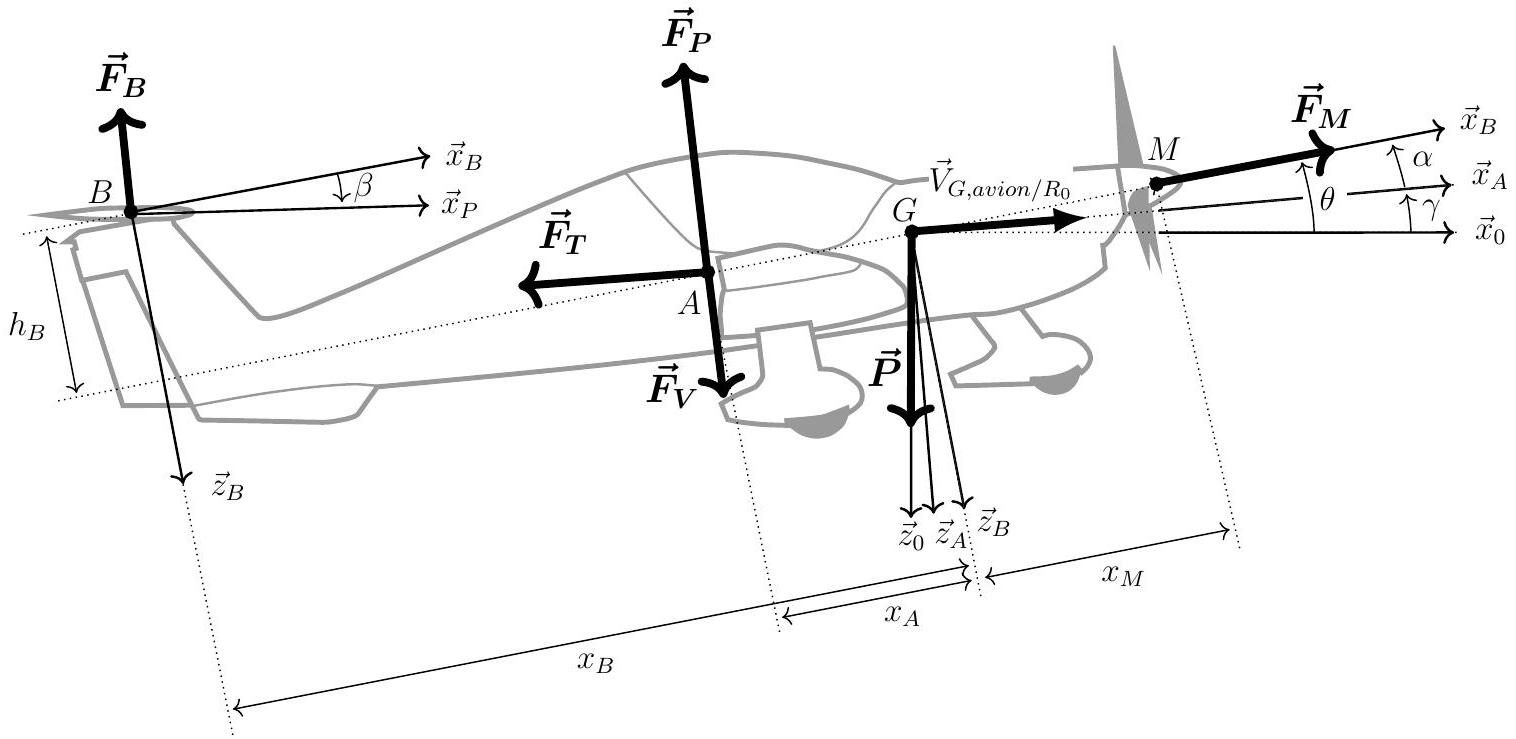
\includegraphics[alt={},max width=\textwidth]{b437a5a5-8562-4c88-96c5-adc15de36bac-04_739_1516_120_269}
\captionsetup{labelformat=empty}
\caption{Figure 4 - Repère et paramétrage associé à l'avion}
\end{center}
\end{figure}

Par ailleurs $\beta=\left(\vec{x}_{B}, \vec{x}_{P}\right)$ représente l'angle d'inclinaison de la gouverne de profondeur (monobloc, en liaison pivot avec le fuselage) par rapport à l'avion.

Les actions mécaniques qui s'appliquent sur l'avion sont

\begin{itemize}
  \item[-] le poids de l'avion s'exerçant au centre de gravité $G: \vec{P}=m g \vec{z}_{0}\left(g=9,81 \mathrm{~m} \cdot \mathrm{~s}^{-2}\right)$;
  \item[-] la force de propulsion de l'hélice s'exerçant au point $M: \vec{F}_{M}=F_{M} \vec{x}_{B}$;
  \item[-] les forces aérodynamiques dues à la vitesse de l'avion qui s'exercent au foyer aérodynamique $A$ des surfaces portantes (ailes et une partie du fuselage) qui se décomposent en deux composantes, une force de portance $\vec{F}_{P}$ et une force de trainée $\vec{F}_{T}$ dans le repère $R_{A}$ :
$$
\vec{F}_{P}=-\frac{1}{2} \rho\left(C_{z_{0}}+C_{z} \alpha\right) S V^{2} \vec{z}_{A} \quad, \quad \vec{F}_{T}=-\frac{1}{2} \rho\left(C_{x_{0}}+C_{x} \alpha\right) S V^{2} \vec{x}_{A}
$$
avec $\rho$ la masse volumique de l'air, $S$ une surface, $C_{z_{0}}, C_{z}, C_{x_{0}}$ et $C_{x}$ des coefficients aérodynamiques caractéristiques de l'avion ;
  \item[-] la force de portance générée par la gouverne de profondeur au centre de poussée $B$ (la force de trainée associée est négligée) où $C_{p_{0}}$ et $C_{p}$ sont des coefficients aérodynamiques caractéristiques de l'avion :
$$
\vec{F}_{B}=-\frac{1}{2} \rho\left[C_{p_{0}}+C_{p}(\alpha+\beta)\right] S V^{2} \vec{z}_{A}
$$
  \item[-] une force perturbatrice qui s'exerce en $A$ et aura pour conséquence une variation d'altitude (par exemple une rafale de vent, l'effet du sol lors d'un atterrissage...) : $\vec{F}_{V}=F_{V} \vec{z}_{A}$.
\end{itemize}

Enfin, les dimensions de l'avion permettent de définir les vecteurs suivants :

$$
\overrightarrow{G A}=-x_{A} \vec{x}_{B} \quad, \quad \overrightarrow{G B}=-x_{B} \vec{x}_{B}-h_{B} \vec{z}_{B} \quad, \quad \overrightarrow{G M}=x_{M} \vec{x}_{B}
$$

\section*{I - Vol de croisière : analyse du régime stationnaire}
Objectif\\
Calculer le point de fonctionnement en régime permanent et vérifier s'il est atteignable au regard des capacités de l'avion.

La conception des lois de commande nécessite de définir un point de fonctionnement et les valeurs des différentes grandeurs associées autour de ce point (vol de croisière pour une vitesse de référence $V_{0}$ et une altitude choisies à priori).

En l'absence de vent, et dans le cas d'un vol stationnaire, l'avion vole à altitude et à vitesses constantes. Dans cette configuration, $F_{V}=0 \mathrm{~N}, V=V_{x}=V_{0}, V_{z}=0 \mathrm{~m} \cdot \mathrm{~s}^{-1}, \beta=0^{\circ}$ et $\gamma=0^{\circ}$.

Q1. En appliquant le Principe Fondamental de la Statique à l'avion, projeté dans le repère aérodynamique $R_{A}$, déterminer la force de propulsion $F_{M}$ en fonction de la vitesse $V$, de l'angle $\alpha$, de la masse volumique de l'air $\rho$ et des constantes caractéristiques de l'avion. Montrer également que la vitesse $V$ vérifie une égalité en fonction uniquement de $\alpha, \rho$ et des constantes caractéristiques de l'avion.

Q2. Afin que l'avion soit en vol stationnaire, montrer que l'angle $\alpha$ doit vérifier une égalité particulière indépendante de la vitesse $V$ de la forme :

$$
1+l_{1} \tan \alpha+\left(l_{2}+l_{3} \tan \alpha\right) \alpha=0
$$

Donner les expressions des termes $l_{1}, l_{2}$ et $l_{3}$.\\
La masse volumique de l'air est un paramètre variant selon l'altitude. Pour la synthèse des lois de commande il est choisi d'utiliser la valeur $\rho=0,8 \mathrm{~kg} \cdot \mathrm{~m}^{-3}$ correspondant à une altitude de croisière de 4000 m , pour laquelle les coefficients aérodynamiques prennent les valeurs suivantes :

$$
C_{x 0}=0,066 \quad C_{x}=0,26 \mathrm{rad}^{-1} \quad C_{z 0}=0,4 \quad C_{z}=11,6 \mathrm{rad}^{-1} \quad C_{p 0}=-0,045 \quad C_{p}=1,08 \mathrm{rad}^{-1} \quad S=8 \mathrm{~m}^{2}
$$

Pour une masse de l'avion $m=630 \mathrm{~kg}$, la résolution de l'équation obtenue question Q2 donne $\alpha=0,84^{\circ}$.\\
Q3. À partir des relations obtenues à la question Q1, calculer la vitesse de croisière $V_{0}$ de l'avion et la force de propulsion $F_{M 0}$. En argumentant la réponse, et compte tenu des capacités de l'avion précisées dans le diagramme d'exigences donné figure 3, déterminer si ce point de fonctionnement $\left(V_{0}, F_{M 0}\right)$ est atteignable.

On notera dans la suite, $\alpha_{0}$ l'angle particulier donné précédemment, $V_{0}$ la vitesse de croisière et $F_{M 0}$ la force de propulsion associée.

\section*{II - Modèles dynamiques, non linéaire et linéaire, de l'avion}
$\_\_\_\_$ Objectif $\_\_\_\_$\\
Définir les modèles dynamiques de l'avion nécessaires à la synthèse et à la validation de la structure de commande du pilote automatique.

La démarche de synthèse et de validation des lois de commande repose sur un ensemble de modèles dynamiques de l'avion. Leur définition s'appuie sur les lois dynamiques régissant le comportement de l'avion autour du point de fonctionnement précédemment déterminé. Les équations dynamiques étant non linéaires, une linéarisation de ces équations sera proposée en se limitant à des développements à l'ordre 1.

Hypothèses : dans la suite, il est supposé que les variations des différentes grandeurs (vitesses, angles, etc.) sont faibles autour de leur position d'équilibre déterminée dans la partie I.

$$
V_{x}=V_{0}+\Delta V_{x} \quad ; \quad V_{z}=\Delta V_{z} \quad ; \quad \gamma=0+\Delta \gamma \quad ; \quad \alpha=\alpha_{0}+\Delta \alpha \quad ; \quad \beta=0+\Delta \beta \quad ; \quad F_{M}=F_{M 0}+\Delta F_{M}
$$

Les notations suivantes sont rappelées :

\begin{itemize}
  \item[-] vecteur position du centre de gravité de l'avion $\overrightarrow{O G}=x(t) \vec{x}_{0}+y(t) \vec{y}_{0}-z(t) \vec{z}_{0}$;
  \item[-] vecteur vitesse de l'avion par rapport au repère terrestre $\vec{V}_{G, \text { avion } / R_{0}}=V(t) \vec{x}_{A}=V_{x}(t) \vec{x}_{0}-V_{z}(t) \vec{z}_{0}$.
\end{itemize}

Q4. Déterminer le vecteur accélération $\vec{\Gamma}_{G, \text { avion } / R_{0}}=\left[\frac{\mathrm{d} \vec{V}_{G, \text { avion } / R_{0}}}{\mathrm{~d} t}\right]_{R_{0}}$ de l'avion par rapport au référentiel galiléen exprimé dans le repère de l'avion $R_{A}$. Avec les hypothèses posées et en négligeant les termes d'ordre 2, en déduire une expression simple de ce vecteur accélération en fonction des dérivées temporelles de $\Delta V_{x}$ et $\Delta V_{z}$.

Q5. Écrire les relations issues du théorème de la résultante dynamique (TRD) appliqué à l'avion, en projection dans le repère $R_{A}$.

Pour la suite, il est admis :

\begin{itemize}
  \item[-] la propriété $V^{2}=V_{x}^{2}+V_{z}^{2}$;
  \item[-] l'équation issue de la question Q1 $F_{M 0} \cos \alpha_{0}-\frac{1}{2} \rho\left(C_{x_{0}}+C_{x} \alpha_{0}\right) S V_{0}^{2}=0$.
\end{itemize}

Q6. Avec les hypothèses et en négligeant les termes d'ordre 2, montrer que l'équation du TRD selon $\vec{x}_{A}$ vérifie une équation différentielle à coefficients constants de la forme :


\begin{equation*}
\frac{\mathrm{d} \Delta V_{x}}{\mathrm{~d} t}+a \Delta V_{x}=-g \Delta \gamma+b \Delta F_{M}-c \Delta \alpha \tag{1}
\end{equation*}


Donner les expressions de $a, b, c$ en fonction de constantes caractéristiques de l'avion, de $\rho, V_{0}, \alpha_{0}$ et $F_{M 0}$ uniquement.

Par une démarche identique, on peut montrer que l'équation du TRD selon $\vec{z}_{A}$ vérifie une équation différentielle à coefficients constants de la forme :


\begin{equation*}
\frac{1}{V_{0}} \frac{\mathrm{~d} \Delta V_{z}}{\mathrm{~d} t}=\frac{\mathrm{d} \Delta \gamma}{\mathrm{~d} t}=d \Delta \alpha+e \Delta \beta+f \Delta V_{x}+h \Delta F_{M}-\frac{1}{m V_{0}} F_{v} \tag{2}
\end{equation*}


Q7. Avec les hypothèses posées et en négligeant les termes d'ordre 2, justifier la relation $\Delta V_{z}=V_{0} \Delta \gamma$.\\
Le comportement dynamique de l'avion est également régi par une équation complémentaire issue du théorème du moment dynamique appliqué à l'avion.\\
La matrice d'inertie au centre de gravité $G$ de l'avion dans son repère $R_{B}$ s'écrit :

$$
\underline{I}_{\text {G,avion }}=\left[\begin{array}{rrr}
I_{1} & 0 & -I_{4} \\
0 & I_{2} & 0 \\
-I_{4} & 0 & I_{3}
\end{array}\right]_{R_{B}}
$$

Q8. Déterminer le moment dynamique en $A$ de l'avion dans le repère $R_{0}$. En négligeant les termes d'ordre 2, simplifier cette expression.

\begin{itemize}
  \item[Q9.] En appliquant le théorème du moment dynamique à l'avion en $A$ projeté sur l'axe $\vec{y}_{0}$, déterminer l'équation du mouvement sans chercher à linéariser cette dernière.
\end{itemize}

Avec les hypothèses du sujet, la relation obtenue à la question précédente peut être linéarisée, conduisant ainsi à une équation différentielle à coefficients constants :


\begin{equation*}
I_{2} \frac{\mathrm{~d}^{2} \Delta \gamma}{\mathrm{~d} t^{2}}+k \frac{\mathrm{~d} \Delta \gamma}{\mathrm{~d} t}-r \Delta \gamma=-I_{2} \frac{\mathrm{~d}^{2} \Delta \alpha}{\mathrm{~d} t^{2}}-l \Delta \alpha-n \Delta \beta+o \frac{\mathrm{~d} \Delta V_{x}}{\mathrm{~d} t}-q \Delta V_{x} \tag{3}
\end{equation*}


\section*{III - Validation du modèle dynamique de l'avion}
Les équations obtenues dans la partie II permettent d'établir deux modèles :

\begin{itemize}
  \item[-] un modèle dit Non Linéaire, découlant des relations du principe fondamental de la dynamique (PFD) avant simplifications avec les hypothèses du sujet;
  \item[-] un modèle dit Linéarisé, découlant des équations 1, 2 et 3.
\end{itemize}

Ces deux modèles sont exploités pour mettre en place un outil de simulation permettant d'obtenir les courbes données dans la figure 15 de l'annexe B. Sur cette figure, les évolutions des grandeurs de sortie (vitesses $V_{x}$ et $V_{z}$ ) sont calculées pour une évolution trapézoïdale de l'angle de la gouverne de profondeur $\beta$ (colonne de gauche) ainsi que pour une évolution en échelon de la force de propulsion $\Delta F_{M}$ (colonne de droite).

Q10. Au vu de ces courbes, commenter les écarts entre les modèles Non Linéaire et Linéarisé. Distinguer les régimes transitoires (fréquences propres, amortissements...) et permanents. Conclure sur le modèle à choisir pour la suite de l'étude.

\section*{Partie B - Étude de la chaine cinématique de la gouverne de profondeur}
La partie précédente a permis d'établir que le changement d'altitude était piloté à partir de l'angle de la gouverne de profondeur $\beta$. Le pilotage de cet angle est réalisé par l'intermédiaire d'un servomoteur et d'un mécanisme dont le schéma cinématique et le paramétrage associé sont donnés en annexe C. À chacun des solides $i$ est associé un repère $R_{i}$, la carlingue de l'avion étant le repère de référence $R_{B}$. Le rotor du servomoteur est lié au solide 3, tandis que la gouverne de profondeur est numérotée 8.

Objectif\\
Déterminer une loi linéaire liant l'angle du servomoteur $\theta_{3}$ à l'angle de la gouverne de profondeur $\beta$.

Q11. À partir du schéma et du paramétrage donné en annexe C, proposer une démarche permettant de déterminer une relation entre $\theta_{3}$ et l'angle de la gouverne de profondeur $\beta$. Aucun calcul n'est attendu à cette question.

Q12. En particulier, déterminer mathématiquement une relation liant les angles $\beta$ et $\theta_{6}$ en fonction des paramètres géométriques du mécanisme. La présenter sous la forme $L_{7}^{2}=(\cdots)^{2}+(\cdots)^{2}$.

Les expressions candidates n'étant pas linéaires, dans la suite il est proposé d'approcher la fonction $\theta_{3}=f\left(\theta_{1}\right)$ numériquement par dichotomie. Il est défini pour cela les fonctions Python :

\begin{verbatim}
from math import *
def loi31(theta3, theta1):
    # Évalue la loi entrée sortie liant les angles theta3 et theta1 pour des valeurs particulières,
    # tel que loi31(theta3,theta1) = 0 si la loi est vérifiée.
    #
    return L2**2-(XD+L3*cos(theta3)-L1*cos(theta1))**2-(-YA+L3*sin(theta3)-L1*sin(theta1))**2
def dichotomie(f, y, xmin, xmax, epsilon):
    # Détermine la valeur de x qui vérifie f(x,y)=0 par dichotomie sur le domaine [xmin, xmax]
    # avec une précision de epsilon sur la valeur de x.
\end{verbatim}

\begin{verbatim}
x = 0.0
# Code à proposer
return x
\end{verbatim}

Par exemple, l'utilisation de la fonction dichotomie(loi31,-1.3,0,np.pi,1e-3) renvoie la valeur 0.829117.\\
Q13. Proposer, directement sur la copie, une procédure écrite en Python pour la fonction dichotomie dont la signature a été définie précédemment et permettant de déterminer la valeur numérique de $\theta_{3}$ pour une valeur particulière de $\theta_{1}$.

La courbe en figure 5, déterminée par dichotomie conformément à la démarche retenue à la Q11, donne l'angle de la gouverne de profondeur $\beta$ en fonction de l'angle du servomoteur $\theta_{3}$.

\begin{figure}[h]
\begin{center}
  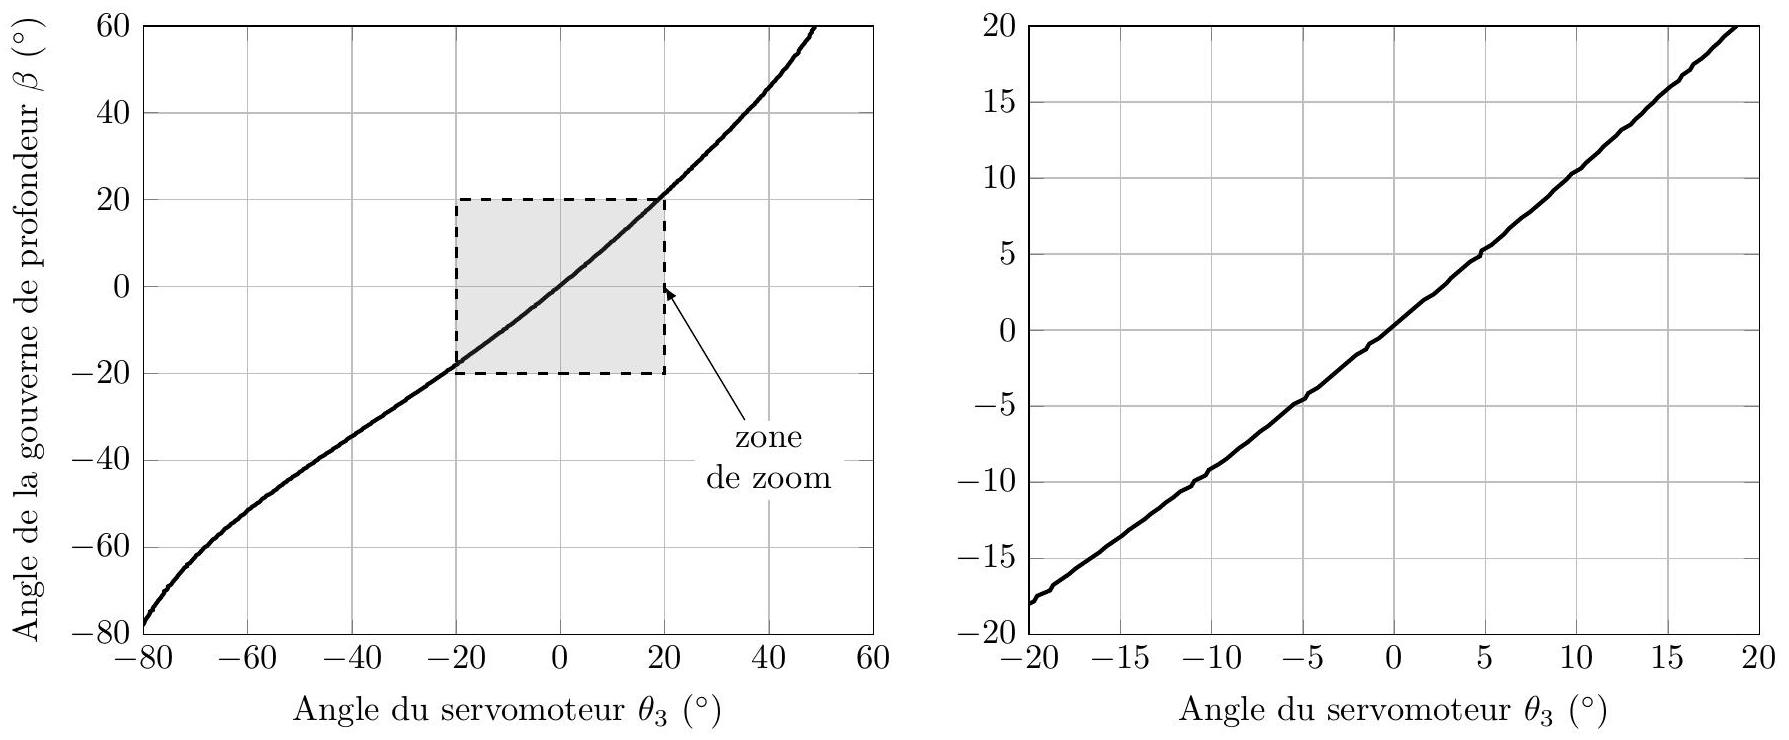
\includegraphics[alt={},max width=\textwidth]{b437a5a5-8562-4c88-96c5-adc15de36bac-08_740_1789_706_148}
\captionsetup{labelformat=empty}
\caption{Figure 5 - Évolution de l'angle $\beta$ en fonction de l'angle du servomoteur $\theta_{3}$ (gauche) et détails (droite)}
\end{center}
\end{figure}

Q14. Au regard de la courbe en figure 5 et compte tenu du domaine de fonctionnement de l'avion, donner l'expression d'une loi linéaire approchée permettant de relier $\beta$ à l'angle $\theta_{3}$. Proposer un indicateur permettant de quantifier l'erreur de modèle commise.

\section*{Partie C - Réglage du pilote automatique}
Les parties précédentes ont permis de déterminer un modèle dynamique de l'avion et un modèle cinématique liant l'angle de la gouverne de profondeur $\beta$ à la position angulaire du rotor du servomoteur $\theta_{3}$ du pilote automatique.

L'avion est équipé d'un ensemble de capteurs et d'une unité de traitement GARMIN GDU460 permettant de déterminer les commandes à envoyer aux servomoteurs.\\
$\_\_\_\_$ Objectif $\_\_\_\_$\\
Régler les paramètres de la loi de commande et vérifier les performances de l'asservissement au regard des exigences du cahier des charges.

Il s'agira dans la suite de concevoir les correcteurs et de régler les différents paramètres des chaines d'asservissement des vitesses verticale et horizontale associées à la structure de commande du pilote automatique.

\section*{I - Définition des modèles pour la conception du pilote automatique}
La phase de modélisation dynamique conduite dans la Partie A a permis d'aboutir à un système de trois équations différentielles linéaires couplées (1, 2 et 3).

Après avoir appliqué les transformées de Laplace à ces équations, elles deviennent :

$$
\begin{aligned}
& (p+a) \Delta V_{x}(p)=-g \Delta \Gamma(p)+b \Delta F_{M}(p)-c \Delta \alpha(p) \\
& p \Delta \Gamma(p)=d \Delta \alpha(p)+e \Delta \beta(p)+f \Delta V_{x}(p)+h \Delta F_{M}(p)-\frac{1}{m V_{0}} F_{v}(p) \\
& \left(I_{2} p^{2}+k p-r\right) \Delta \Gamma(p)=-\left(I_{2} p^{2}+l\right) \Delta \alpha(p)-n \Delta \beta(p)+(o p-q) \Delta V_{x}(p)
\end{aligned}
$$

où $\Delta V_{x}(p), \Delta \Gamma(p), \Delta F_{M}(p), \Delta \alpha(p), \Delta \beta(p)$ et $F_{v}(p)$ sont les transformées de Laplace respectives des grandeurs temporelles $\Delta V_{x}(t), \Delta \gamma(t), \Delta F_{M}(t), \Delta \alpha(t), \Delta \beta(t)$ et $F_{v}(t)$.\\
En considérant que l'effort de perturbation $F_{v}(p)$ est nul, et en rappelant la relation $\Delta V_{z}(t)=V_{0} \Delta \gamma(t)$, le modèle dynamique linéarisé peut être représenté par quatre fonctions de transfert :

$$
H_{1}(p)=\left[\frac{\Delta V_{x}(p)}{\Delta F_{M}(p)}\right]_{\Delta \beta(p)=0}, H_{2}(p)=\left[\frac{\Delta V_{z}(p)}{\Delta F_{M}(p)}\right]_{\Delta \beta(p)=0}, H_{3}(p)=\left[\frac{\Delta V_{x}(p)}{\Delta \beta(p)}\right]_{\Delta F_{M}(p)=0}, H_{4}(p)=\left[\frac{\Delta V_{z}(p)}{\Delta \beta(p)}\right]_{\Delta F_{M}(p)=0} .
$$

La structure de la régulation des vitesses horizontale et verticale de l'avion associée au modèle dynamique linéarisé peut ainsi être modélisé par le schéma-bloc donné sur la figure 6.

\begin{itemize}
  \item[-] $\Delta V_{x}^{*}(p)$ et $\Delta V_{z}^{*}(p)$ sont respectivement les variations de consigne des vitesses horizontale et verticale;
  \item[-] $C_{H x}(p)$ et $C_{H z}(p)$ sont les fonctions de transfert respectives des correcteurs pour les boucles d'asservissement en vitesse horizontale et verticale;
  \item[-] $\Delta F_{M}^{*}(p)$ est la variation de consigne de la force de propulsion et $\Delta F_{M}(p)$ est la variation réelle de la force de propulsion;
  \item[-] $H_{m}(p)$ est la fonction de transfert de l'ensemble de la chaine de propulsion;
  \item[-] $\Delta \beta^{*}(p)$ est la variation de consigne de l'angle de gouverne de profondeur et $\Delta \beta(p)$ est la variation de l'angle de la gouverne de profondeur ;
  \item[-] $K_{t}$ est le gain de la chaine cinématique de la gouverne de profondeur et $H_{t}(p)$ est la fonction de transfert de la motorisation associée.
\end{itemize}

\begin{figure}[h]
\begin{center}
  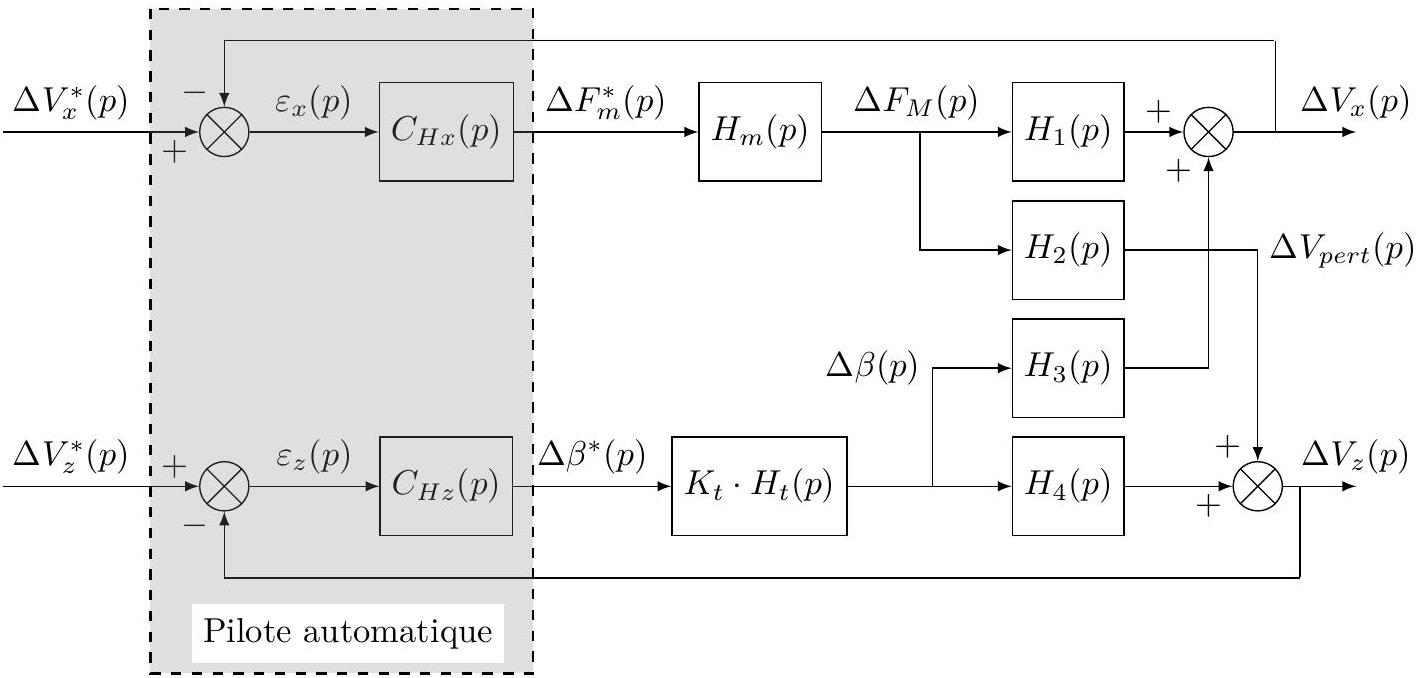
\includegraphics[alt={},max width=\textwidth]{b437a5a5-8562-4c88-96c5-adc15de36bac-09_678_1417_1414_313}
\captionsetup{labelformat=empty}
\caption{Figure 6 - Schéma-bloc couplé de l'asservissement des vitesses horizontale et verticale}
\end{center}
\end{figure}

Le schéma-bloc met en évidence le couplage entre les différentes variables et montre ainsi que $\Delta V_{x}(p)$ et $\Delta V_{z}(p)$ sont simultanément influencées par $\Delta V_{x}^{*}(p)$ et $\Delta V_{z}^{*}(p)$. Les hypothèses suivantes sont adoptées pour la suite :

\begin{itemize}
  \item[-] la fonction de transfert de la motorisation de la gouverne de profondeur, au vu de la technologie et de la rapidité de l'actionneur retenu, peut être considérée comme unitaire $H_{t}(p)=1$;
  \item[-] quels que soient les résultats obtenus dans la partie précédente, le gain de la chaine cinématique de la gouverne de profondeur est unitaire $K_{t}=1$.
\end{itemize}

Le cahier des charges associé à cet asservissement est donné dans le diagramme d'exigences, figure 3.

\section*{II - Asservissement en vitesse verticale $V_{z}$}
Objectif

Régler le correcteur de vitesse verticale $V_{z}$ compte tenu de la dépendance entre les forces aérodynamiques et la vitesse de l'avion.

Dans un premier temps, seul l'asservissement en vitesse verticale est pris en compte, en exploitant le modèle linéarisé et en supposant que la variation de vitesse verticale est découplée. L'effet du couplage est ainsi assimilé dans ce cas à un signal perturbateur extérieur $\Delta V_{\text {pert }}(p)$. La boucle d'asservissement est alors représentée par le schéma-bloc de la figure 7.

\begin{figure}[h]
\begin{center}
  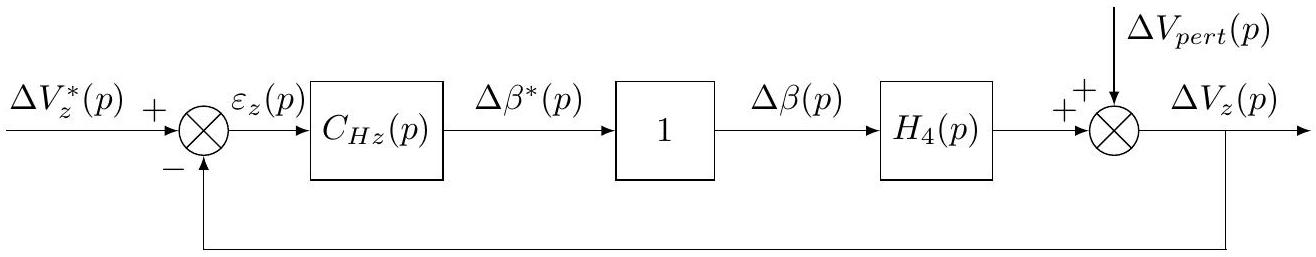
\includegraphics[alt={},max width=\textwidth]{b437a5a5-8562-4c88-96c5-adc15de36bac-10_257_1316_476_373}
\captionsetup{labelformat=empty}
\caption{Figure 7 - Boucle de vitesse verticale linéarisée et découplée}
\end{center}
\end{figure}

La structure du correcteur est de type proportionnel intégral de fonction de transfert $C_{H z}(p)=K_{z}\left(1+\frac{1}{\tau_{z} p}\right)$, avec $K_{z}<0$.

\begin{figure}[h]
\begin{center}
  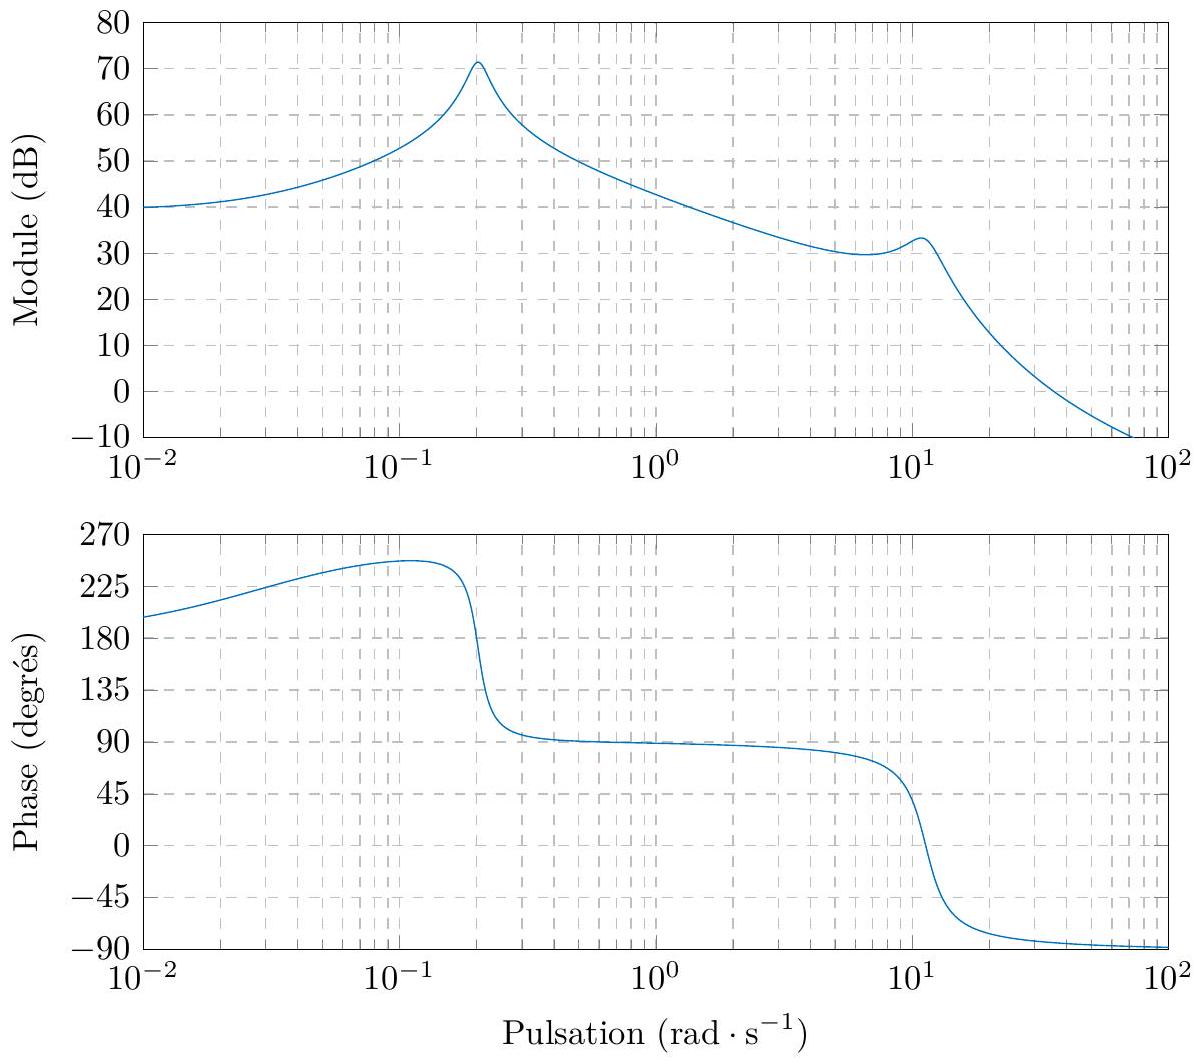
\includegraphics[alt={},max width=\textwidth]{b437a5a5-8562-4c88-96c5-adc15de36bac-10_1063_1200_1054_431}
\captionsetup{labelformat=empty}
\caption{Figure 8 - Diagramme de Bode de la fonction de transfert $H_{4}(p)$}
\end{center}
\end{figure}

Le diagramme de Bode de la fonction de transfert $H_{4}(p)$ est donné sur la figure 8. Le temps de réponse à 5 \% attendu pour la boucle d'asservissement de la vitesse verticale est d'environ 5 secondes. L'exploitation des relations approchées usuelles liant la pulsation de coupure à 0 dB et le temps de réponse en boucle fermée permet de restreindre la plage d'étude fréquentielle au voisinage de $1 \mathrm{rad} \cdot \mathrm{s}^{-1}$. Le calcul des paramètres du correcteur sera alors effectué dans l'intervalle $\left[0,5 \mathrm{rad} \cdot \mathrm{s}^{-1} ; 5 \mathrm{rad} \cdot \mathrm{s}^{-1}\right]$.

Pour la détermination de $\tau_{z}$, une expression approchée $\tilde{H}_{4}(p)$ de $H_{4}(p)$ est envisagée ainsi que l'utilisation de l'approximation $\omega_{c} t_{r} \simeq 3$, où $\omega_{c}$ est la pulsation de coupure à 0 dB de la fonction de transfert en boucle ouverte et $t_{r}$ le temps de réponse à 5\% en boucle fermée.

\begin{itemize}
  \item[Q15.] Montrer, à partir du diagramme de Bode de la fonction $H_{4}(p)$ donné sur la figure 8, que la fonction $H_{4}(p)$ peut être assimilée à une fonction de la forme $\tilde{H}_{4}(p)=-\frac{K_{4 a}}{p}$, avec $K_{4 a}>0$, dans l'intervalle de pulsations retenu. Donner la valeur de $K_{4 a}$.
  \item[Q16.] Préciser sous forme littérale la fonction de transfert en boucle ouverte en adoptant la forme approchée $\tilde{H}_{4}(p)$. Justifier la valeur négative retenue pour $K_{z}$.
  \item[Q17.] Déterminer, à partir de l'expression de la fonction de transfert de la boucle ouverte, l'expression que doit vérifier $\tau_{z}$ afin de répondre au critère de marge de phase du cahier des charges au regard du temps de réponse souhaité. Faire l'application numérique.
  \item[Q18.] En conservant la valeur de $\tau_{z}$ déterminée à la question Q17 déterminer l'expression de $K_{z}$ permettant de vérifier les critères de marge de phase et de rapidité du cahier des charges. Faire l'application numérique.
\end{itemize}

Le diagramme de Bode de la fonction de transfert en boucle ouverte corrigée établi à partir de la fonction $H_{4}(p)$ et du correcteur $C_{H z}(p)$ déterminé aux questions précédentes est donné sur la figure 9.

\begin{figure}[h]
\begin{center}
  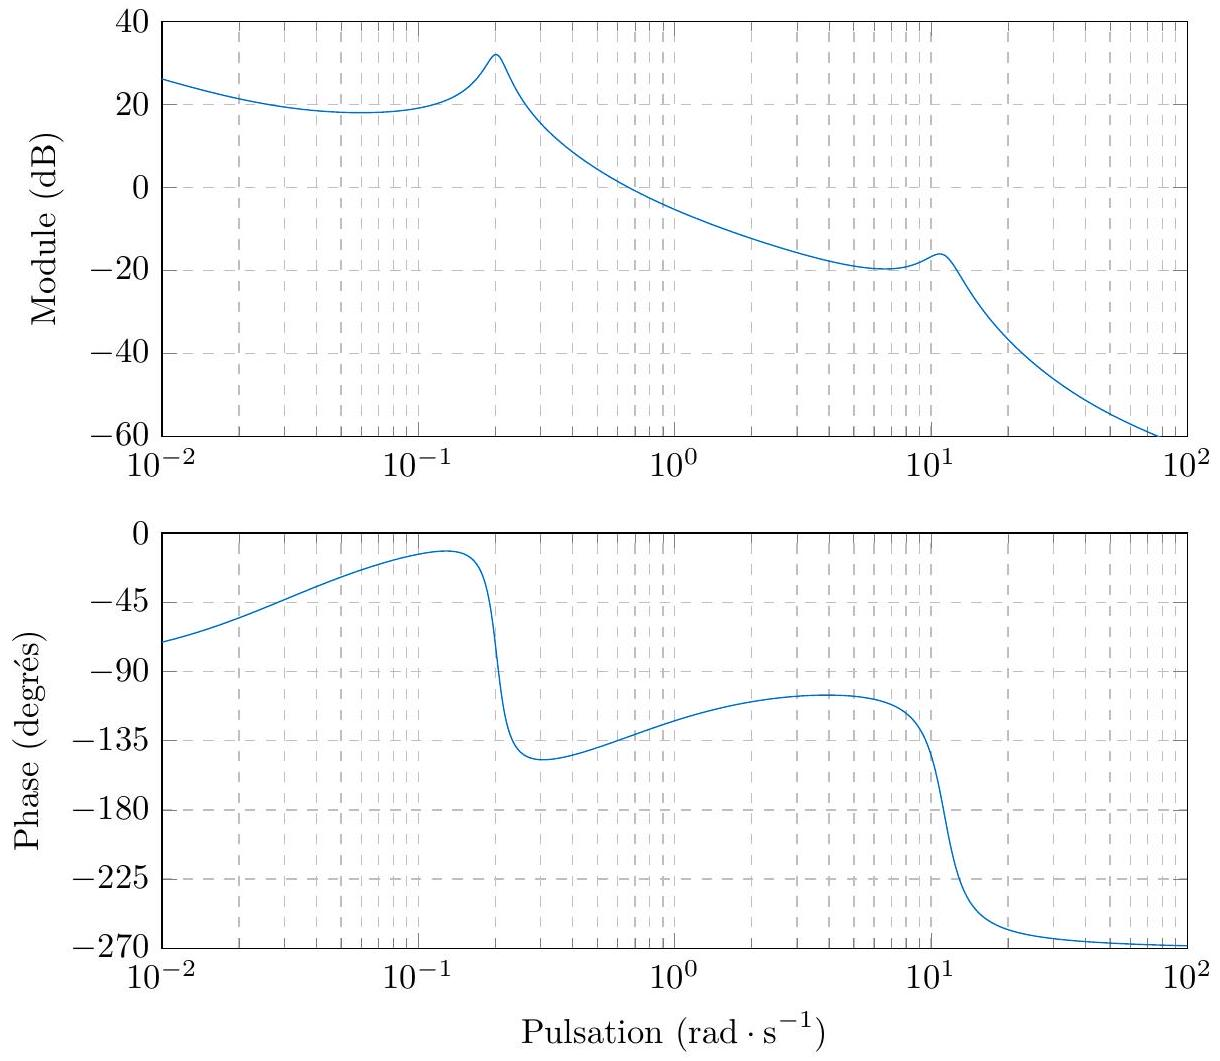
\includegraphics[alt={},max width=\textwidth]{b437a5a5-8562-4c88-96c5-adc15de36bac-12_1061_1220_255_421}
\captionsetup{labelformat=empty}
\caption{Figure 9 - Diagramme de Bode de la fonction de transfert en boucle ouverte corrigée}
\end{center}
\end{figure}

Q19. Déterminer, à partir de ce diagramme de Bode, les marges de gain et de phase. Conclure quant à la pertinence de la loi de commande déterminée pour l'asservissement de la vitesse verticale $V_{z}$.

\section*{III - Asservissement en vitesse horizontale $V_{x}$}
\section*{III. 1 - Fonction de transfert représentative pour la chaine d'asservissement de vitesse horizontale $V_{x}$}
$\_\_\_\_$ Objectif $\_\_\_\_$\\
Exprimer une fonction de transfert simplifiée de la boucle ouverte de l'asservissement de vitesse horizontale, utilisable dans le cadre de la synthèse du correcteur de cette même boucle.

Pour la synthèse du correcteur de la chaine d'asservissement horizontale il est envisagé d'utiliser un modèle simplifié issu de la réduction du schéma-bloc couplé donné à la figure 6 de façon à considérer $\Delta V_{x}^{*}(p)$ comme la consigne de variation de vitesse horizontale et d'assimiler $\Delta V_{z}^{*}(p)$ à une perturbation.

La boucle d'asservissement de la variation de vitesse verticale linéarisée et découplée est représentée sous forme de schéma-bloc sur la figure 7.

Q20. Exprimer la fonction de transfert de la boucle fermée de l'asservissement de vitesse verticale découplée, notée $H_{B F v_{z}}(p)$, en fonction de $H_{4}(p)$ et $C_{H z}(p)$.

Dans le cadre de l'étude de l'asservissement de $\Delta V_{x}$, le schéma bloc de la figure 6 peut se ramener sous la forme du schéma bloc intermédiaire de la figure 10.

Q21. Déterminer l'expression de $A(p)$ en fonction de $H_{4}(p)$ et $H_{B F v_{z}}(p)$ permettant le passage du schéma bloc de la figure 6 au schéma bloc de la figure 10.

\begin{figure}[h]
\begin{center}
  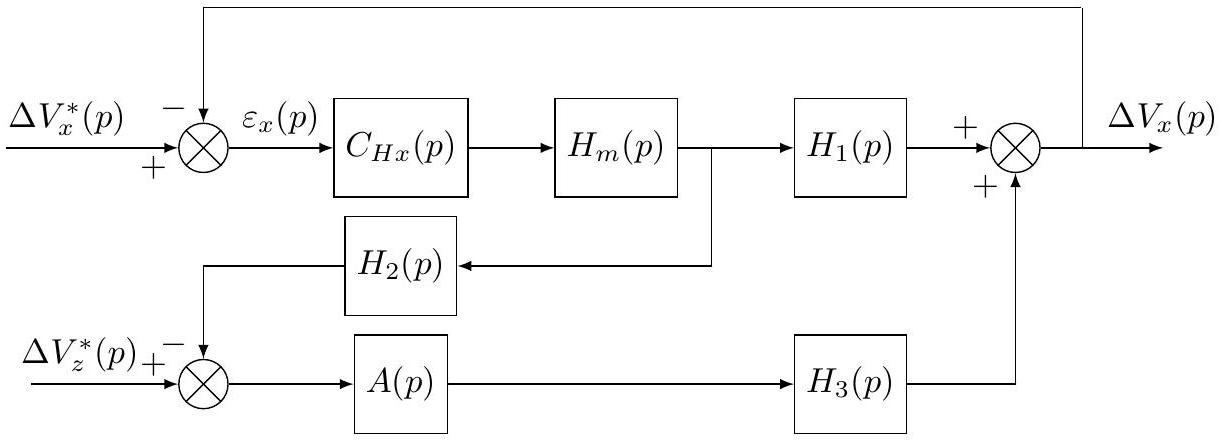
\includegraphics[alt={},max width=\textwidth]{b437a5a5-8562-4c88-96c5-adc15de36bac-13_440_1222_144_414}
\captionsetup{labelformat=empty}
\caption{Figure 10 - Schéma-bloc intermédiaire}
\end{center}
\end{figure}

Q22. Montrer enfin, à partir de la forme précédente donnée figure 10, que le schéma-bloc couplé peut se mettre sous la forme de la figure 11. Donner l'expression de $B(p)$ en fonction de $H_{4}(p), H_{2}(p), H_{3}(p)$ et $H_{B F v_{z}}(p)$.

\begin{figure}[h]
\begin{center}
  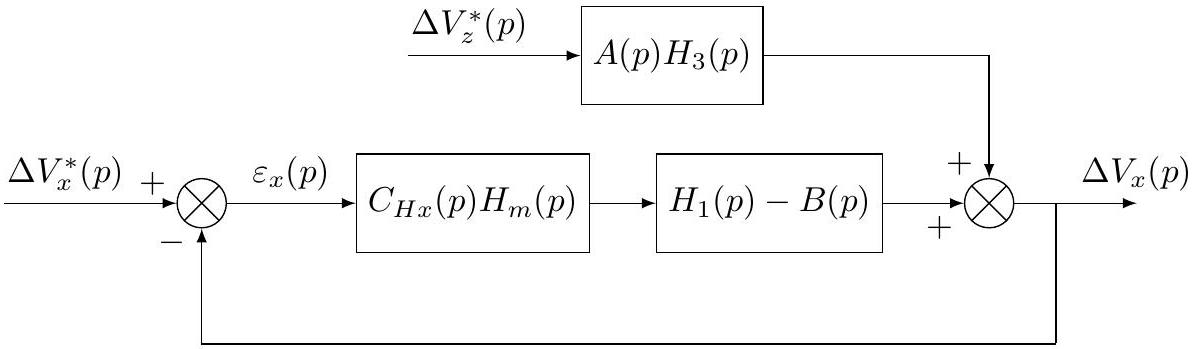
\includegraphics[alt={},max width=\textwidth]{b437a5a5-8562-4c88-96c5-adc15de36bac-13_349_1193_880_428}
\captionsetup{labelformat=empty}
\caption{Figure 11 - Boucle de vitesse horizontale perturbée}
\end{center}
\end{figure}

Le schéma-bloc mis sous la forme de la figure 11 permet ainsi d'exprimer la fonction de transfert en boucle ouverte de l'asservissement de vitesse horizontale $H_{B O v_{x}}(p)=\frac{\Delta V_{x}(p)}{\varepsilon_{x}(p)}$ :

$$
H_{B O v_{x}}(p)=C_{H x}(p) H_{m}(p)\left(H_{1}(p)-B(p)\right)
$$

Le temps de réponse à 5\% attendu pour la boucle d'asservissement de la vitesse horizontale est d'environ 3 secondes. En conséquence, dans le cadre du réglage du correcteur, le modèle de la caractéristique fréquentielle du système au voisinage de $1 \mathrm{rad} \cdot \mathrm{s}^{-1}$, plus précisément entre $0,8 \mathrm{rad} \cdot \mathrm{s}^{-1}$ et $8 \mathrm{rad} \cdot \mathrm{s}^{-1}$, sera plus particulièrement considéré.

La figure 16, annexe D, représente le diagramme de Bode de la fonction de transfert $H_{1}(p)-B(p)$.\\
Q23. Déterminer une expression numérique simplifiée de $H_{1}(p)-B(p)$, notée $\tilde{H}_{1}(p)$, sous la forme $\tilde{H}_{1}(p)=\frac{K_{1 a}}{p}$ $\left(K_{1 a}>0\right)$, utilisable pour le réglage du correcteur de la boucle de variation de vitesse horizontale.

\section*{III. 2 - Synthèse du correcteur de la boucle de vitesse horizontale $V_{x}$}
Objectif\\
Déterminer les paramètres d'un correcteur permettant à la boucle d'asservissement de la vitesse horizontale d'atteindre les objectifs fixés par le cahier des charges fonctionnel.

L'architecture de correcteur retenue pour la boucle de vitesse horizontale est de type proportionnel intégral de fonction de transfert $C_{H x}(p)=K_{x}\left(1+\frac{1}{\tau_{x} p}\right)$.

En phase de vol, le modèle de comportement du groupe de propulsion est approché par celui d'une fonction du premier ordre de gain statique unitaire et de constante de temps 0,01 s :

$$
H_{m}(p)=\frac{1}{1+0,01 p}
$$

\begin{itemize}
  \item[Q24.] Justifier que, dans l'intervalle de pulsations retenu pour le réglage du correcteur, la fonction de transfert en boucle ouverte de l'asservissement de vitesse horizontale $H_{B O v_{x}}(p)$ peut se mettre sous la forme $H_{B O v_{x}}(p)=$ $C_{H x}(p) \tilde{H}_{1}(p)$.
  \item[Q25.] À partir du schéma-bloc simplifié donné en figure 11, en considérant que $H_{1}(p)-B(p)=\tilde{H}_{1}(p)=\frac{K_{1 a}}{p}$, déterminer l'expression littérale sous forme canonique de la fonction de transfert en boucle fermée de la régulation de vitesse horizontale $H_{B F v_{x}}(p)=\frac{\Delta V_{x}(p)}{\Delta V_{x}^{*}(p)}$, en fonction de $K_{1 a}, K_{x}$ et $\tau_{x}$. Conclure quant à la stabilité de la boucle fermée de vitesse horizontale.
  \item[Q26.] Écrire $H_{B F v_{x}}(p)$ sous une forme $H_{B F v_{x}}(p)=X(p)+T p \cdot X(p)$ et donner l'expression de $T$.
  \item[Q27.] Exprimer les paramètres caractéristiques de $X(p)$ : pulsation propre $\omega_{0}$ et coefficient d'amortissement $\xi$. Donner l'expression de $K_{x}$ en fonction de $K_{1 a}$ et $\tau_{x}$, afin que la réponse indicielle de $X(p)$ soit la plus rapide possible, sans dépassement.
\end{itemize}

La figure 12 donne l'abaque du temps de réponse réduit pour les systèmes du deuxième ordre.

\begin{figure}[h]
\begin{center}
  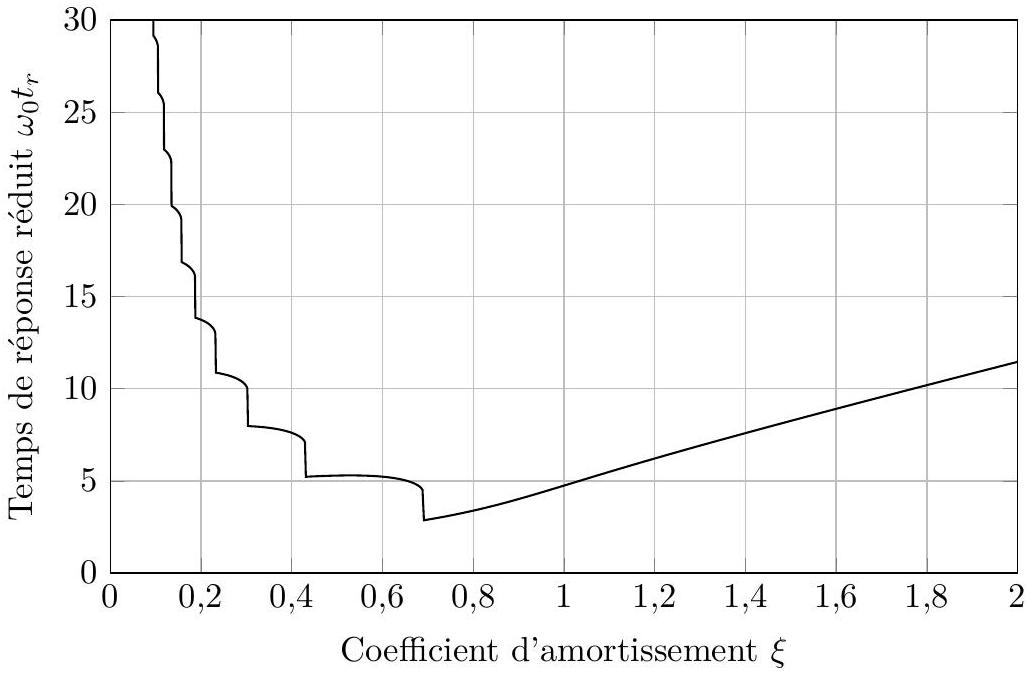
\includegraphics[alt={},max width=\textwidth]{b437a5a5-8562-4c88-96c5-adc15de36bac-14_674_1030_892_510}
\captionsetup{labelformat=empty}
\caption{Figure 12 - Abaque du temps de réponse réduit pour les systèmes du deuxième ordre}
\end{center}
\end{figure}

\begin{itemize}
  \item[Q28.] Donner la valeur de $\tau_{x}$ pour que le temps de réponse à $5 \%$ de la réponse indicielle de $X(p)$ soit de 3 s. En déduire la valeur de $K_{x}$.
\end{itemize}

La figure 17 de l'annexe D représente le tracé de la réponse indicielle de la fonction

$$
\frac{\tau_{x} p}{1+\tau_{x} p+\frac{\tau_{x}}{K_{1 a} K_{x}} p^{2}}=T p \cdot X(p)
$$

\begin{itemize}
  \item[Q29.] Tracer sur la copie la réponse indicielle de $X(p)$ en justifiant la construction de la courbe. À l'aide de la figure 17 de l'annexe D, la compléter avec le tracé de la réponse indicielle de $H_{B F v_{x}}(p)$. Commenter l'influence du zéro de $H_{B F v_{x}}(p)$ sur le comportement temporel.
\end{itemize}

\section*{Partie D - Synthèse}
\section*{I - Robustesse des asservissements en vitesse}
$\_\_\_\_$ Objectif $\_\_\_\_$\\
Valider les performances globales après implémentation des réglages précédents dans le système de commande du pilote automatique.

Pour valider la loi de commande étudiée précédemment il est utilisé un simulateur non linéaire exploitant les modèles dynamiques, couplés, définis précédemment et les correcteurs synthétisés. Une simulation est réalisée sur un intervalle de temps de 50 s au cours duquel les variations de vitesses horizontale et verticale de l'avion sont relevées autour d'un point de fonctionnement défini par $V_{x}(t=0)=60 \mathrm{~m} \cdot \mathrm{~s}^{-1}, V_{z}(t=0)=0$. L'altitude initiale est $z(t=0)=4000 \mathrm{~m}$ et :

\begin{itemize}
  \item[-] à $t=10 \mathrm{~s}$ est imposé un échelon de variation de vitesse horizontale d'amplitude $10 \mathrm{~m} \cdot \mathrm{~s}^{-1}$;
  \item[-] à $t=30 \mathrm{~s}$ est imposé un échelon de variation de vitesse verticale d'amplitude $-3 \mathrm{~m} \cdot \mathrm{~s}^{-1}$.
\end{itemize}

Les évolutions des vitesses horizontale et verticale de l'avion sont données figure 13.

\begin{figure}[h]
\begin{center}
  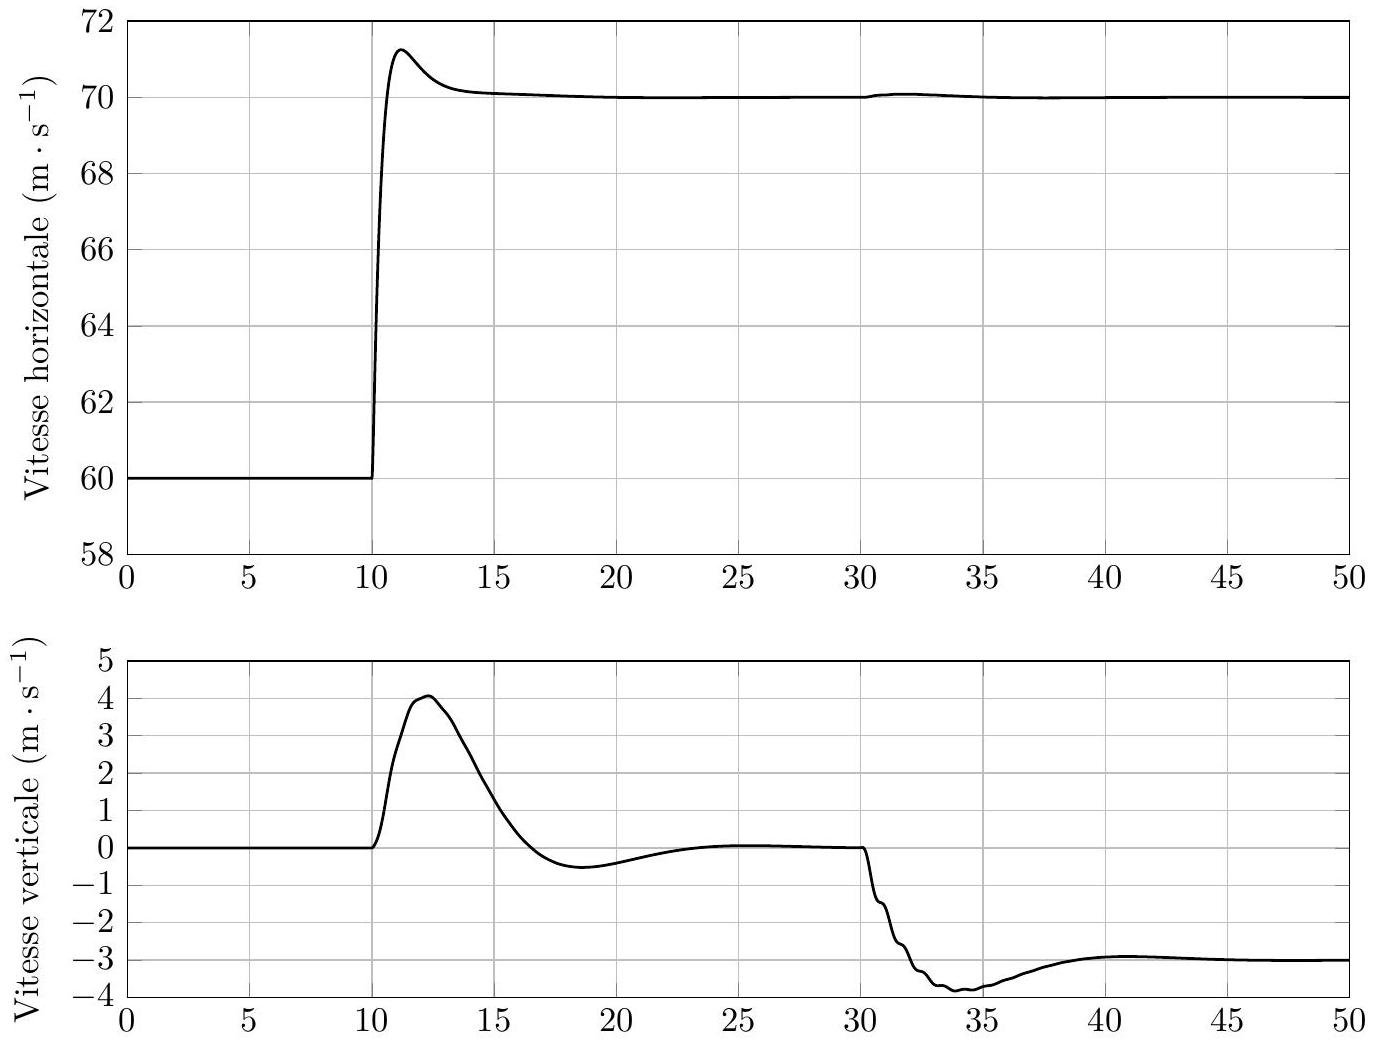
\includegraphics[alt={},max width=\textwidth]{b437a5a5-8562-4c88-96c5-adc15de36bac-15_1042_1374_546_339}
\captionsetup{labelformat=empty}
\caption{Figure 13 - Évolutions des vitesses horizontale et verticale obtenues en simulation numérique avec le modèle non linéaire}
\end{center}
\end{figure}

Q30. À partir des résultats figure 13, commenter les performances des asservissements des vitesses verticale et horizontale. Est-il possible de considérer le comportement de l'avion en fonctionnement « pilote automatique » comme découplé?

\section*{II - Sensibilité du système aux variations de la masse volumique de l'air}
$\_\_\_\_$ Objectif $\_\_\_\_$\\
Quantifier la sensibilité du système aux variations d'un paramètre extérieur : la masse volumique de l'air en fonction de l'altitude. Vérifier la robustesse vis-à-vis de la variation de ce paramètre.

La masse volumique de l'air, de par son rôle dans les forces aérodynamiques, est un paramètre important pour la modélisation du comportement dynamique de l'avion et pour le réglage du système de commande. Le calcul des paramètres des correcteurs a été effectué en considérant une masse volumique de l'air égale à $0,8 \mathrm{~kg} \cdot \mathrm{~m}^{-3}$, valeur mesurée à l'altitude de croisière. Étant donné la forte variation de cette valeur avec l'altitude, il est judicieux d'étudier la sensibilité des performances de la loi de commande vis-à-vis de la masse volumique de l'air, de $1,22 \mathrm{~kg} \cdot \mathrm{~m}^{-3}$ au niveau du sol, à $0,4 \mathrm{~kg} \cdot \mathrm{~m}^{-3}$ à une altitude de 10000 m, supérieure à l'altitude maximale autorisée de l'avion.

Pour cela les modèles en boucle fermée sont déterminés pour différentes valeurs de masse volumique de l'air $\rho \in$ $[0,4 ; \cdots ; 1,22] \mathrm{kg} \cdot \mathrm{m}^{-3}$. De cette étude découle l'évolution des pôles du système \{avion + pilote automatique\}, visible sur le graphique de la figure 14 (cette courbe est appelée lieu des pôles), selon l'évolution de la valeur de masse volumique de l'air.

\begin{figure}[h]
\begin{center}
  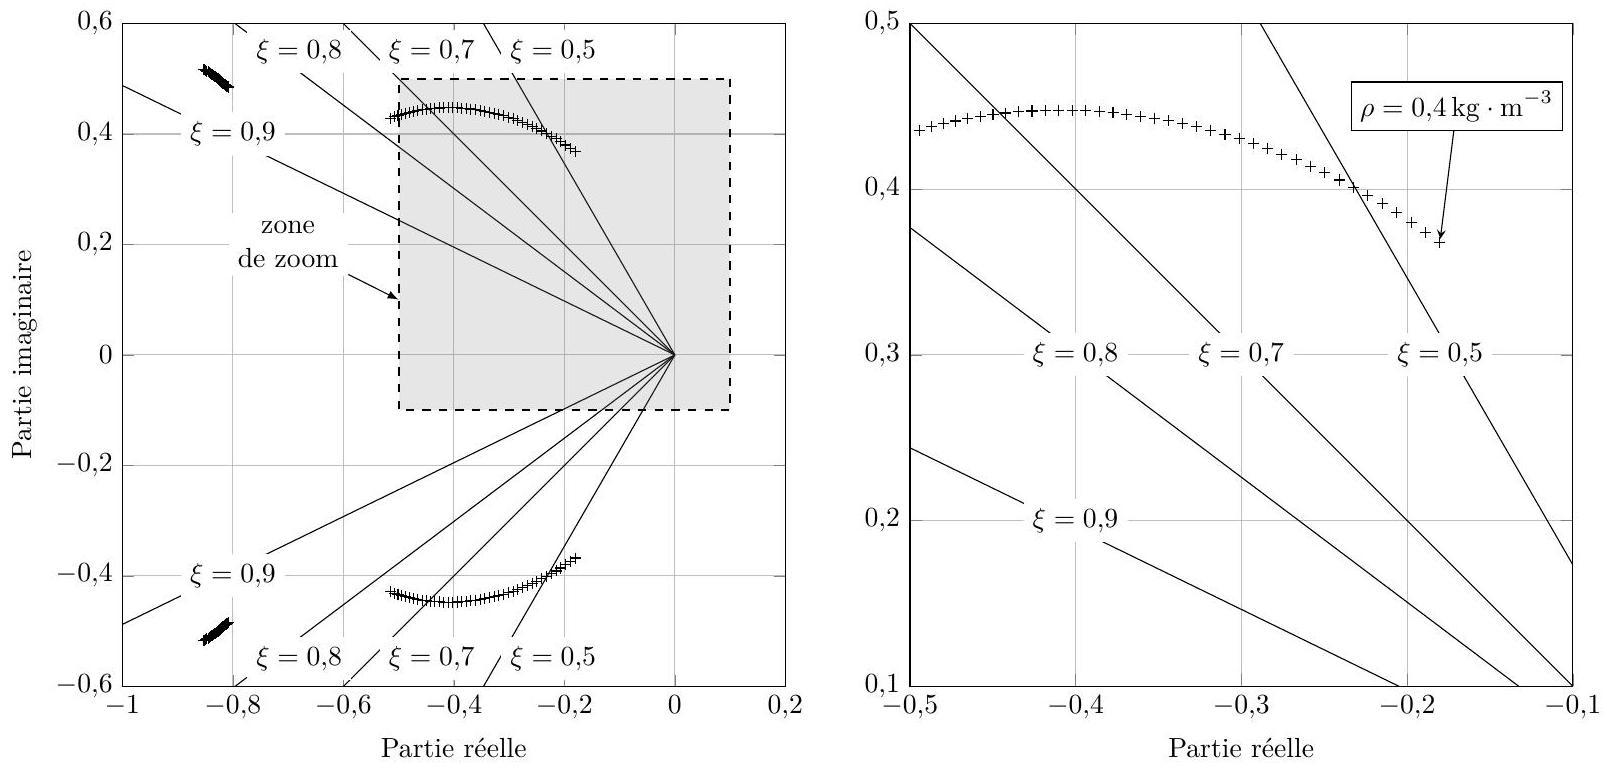
\includegraphics[alt={},max width=\textwidth]{b437a5a5-8562-4c88-96c5-adc15de36bac-16_770_1607_125_221}
\captionsetup{labelformat=empty}
\caption{Figure 14 - Lieu des pôles du système \{avion + pilote automatique\} selon la valeur de masse volumique de l'air (gauche) et détails (droite)}
\end{center}
\end{figure}

Sur la figure 14 le lieu des pôles est représenté par des croix. Le lieu contient les pôles calculés pour une masse volumique de l'air allant de $1,22 \mathrm{~kg} \cdot \mathrm{~m}^{-3}$ à $0,4 \mathrm{~kg} \cdot \mathrm{~m}^{-3}$ avec un pas de $0,02 \mathrm{~kg} \cdot \mathrm{~m}^{-3}$. Les droites obliques sont appelées lignes iso-amortissement. Chaque paire de droites correspond au lieu des pôles d'un système du deuxième ordre avec $\xi \in\{0,5 ; 0,7 ; 0,8 ; 0,9\}$.

\begin{itemize}
  \item[Q31.] En analysant la figure 14, commenter l'évolution du comportement de l'avion en fonction de l'altitude. Proposer des solutions afin de garantir un meilleur comportement global quelle que soit l'altitude.
\end{itemize}

\begin{center}
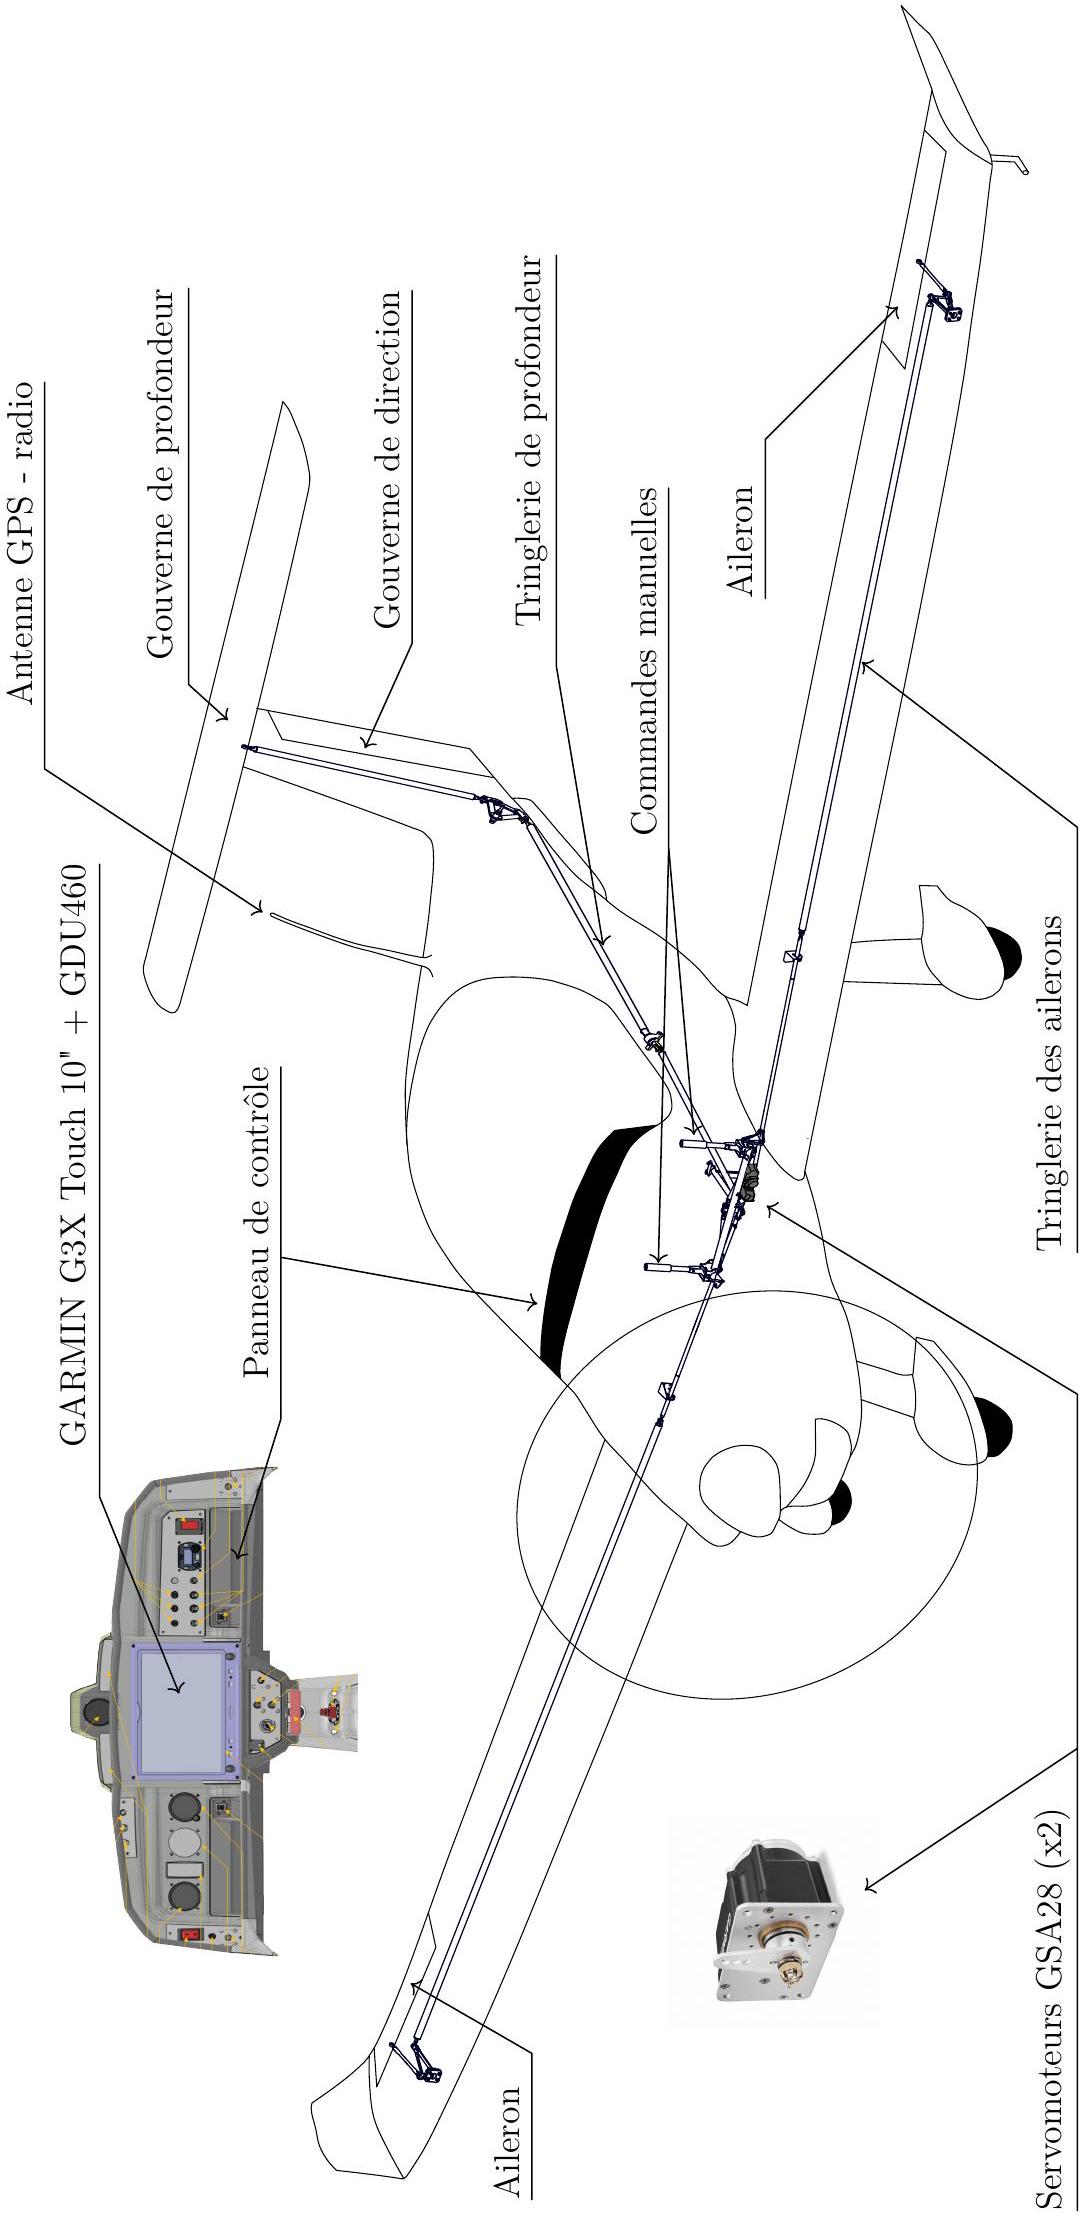
\includegraphics[max width=\textwidth, alt={}]{b437a5a5-8562-4c88-96c5-adc15de36bac-17_2216_1086_267_448}
\end{center}

\section*{Annexe B Comparaison des réponses des modèles Non Linéaire et Linéarisé}
\begin{figure}[h]
\begin{center}
  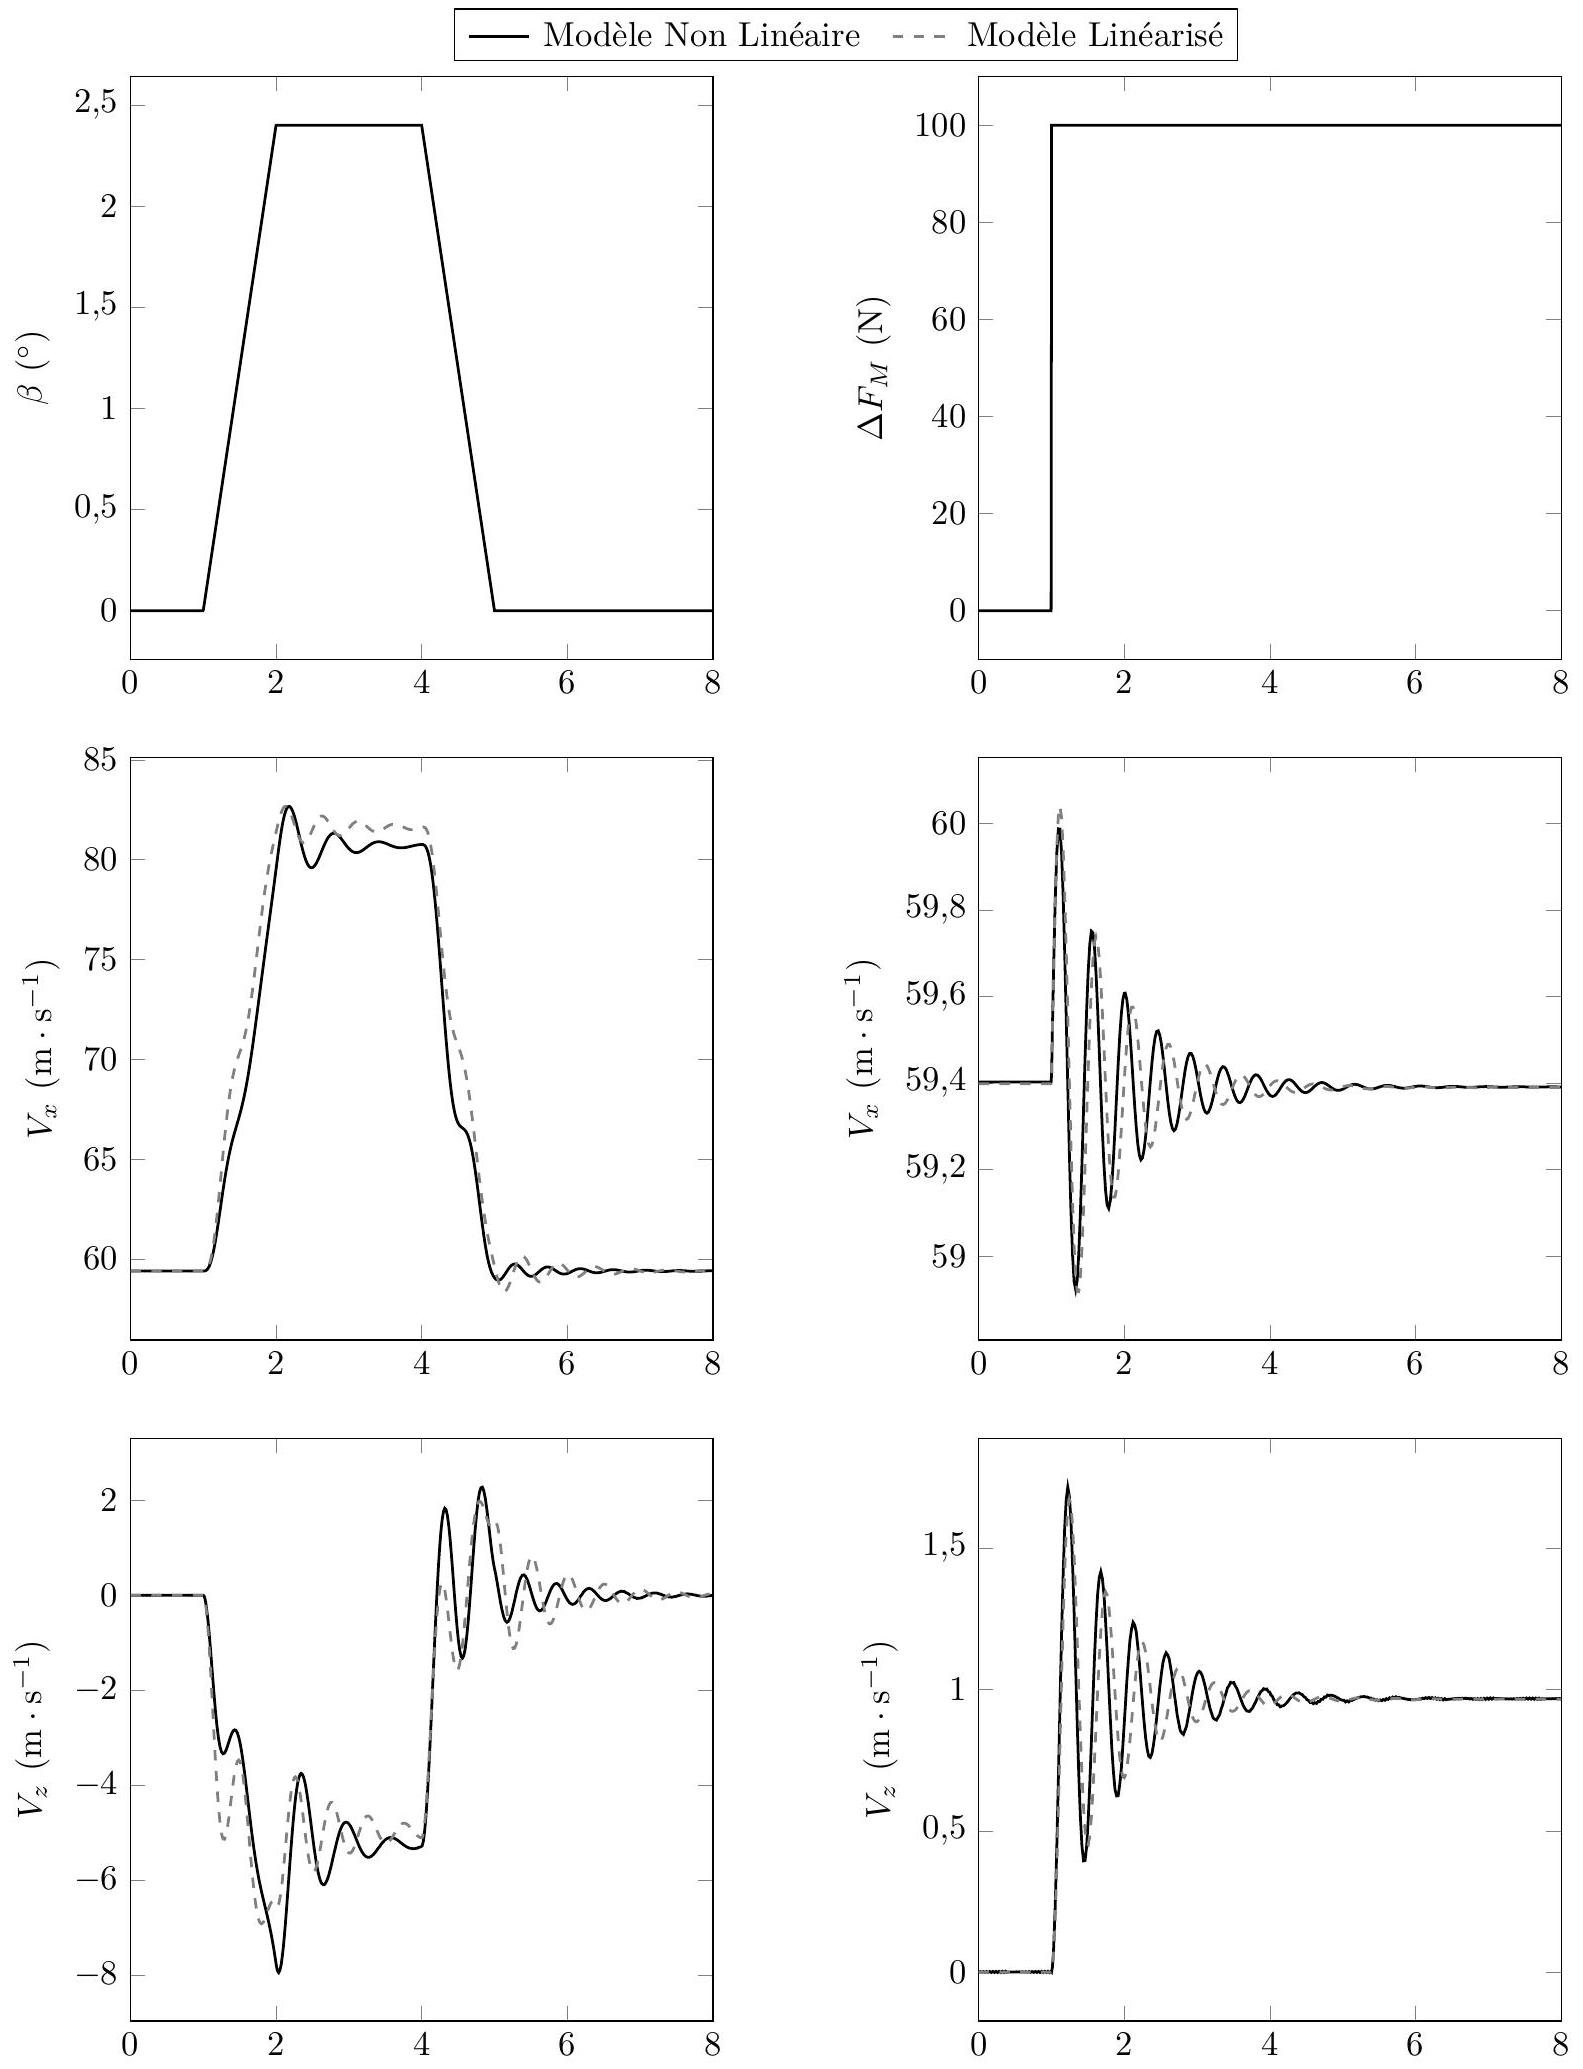
\includegraphics[alt={},max width=\textwidth]{b437a5a5-8562-4c88-96c5-adc15de36bac-18_2069_1583_289_236}
\captionsetup{labelformat=empty}
\caption{Figure 15 - Comparaison des modèles Non Linéaire (NL) et Linéarisé (L) en fonction des entrées $\beta$ (gauche) et $\Delta F_{m}$ (droite)}
\end{center}
\end{figure}

\section*{Annexe C Schéma cinématique du mécanisme d'orientation de la gouverne de profondeur}
\begin{center}
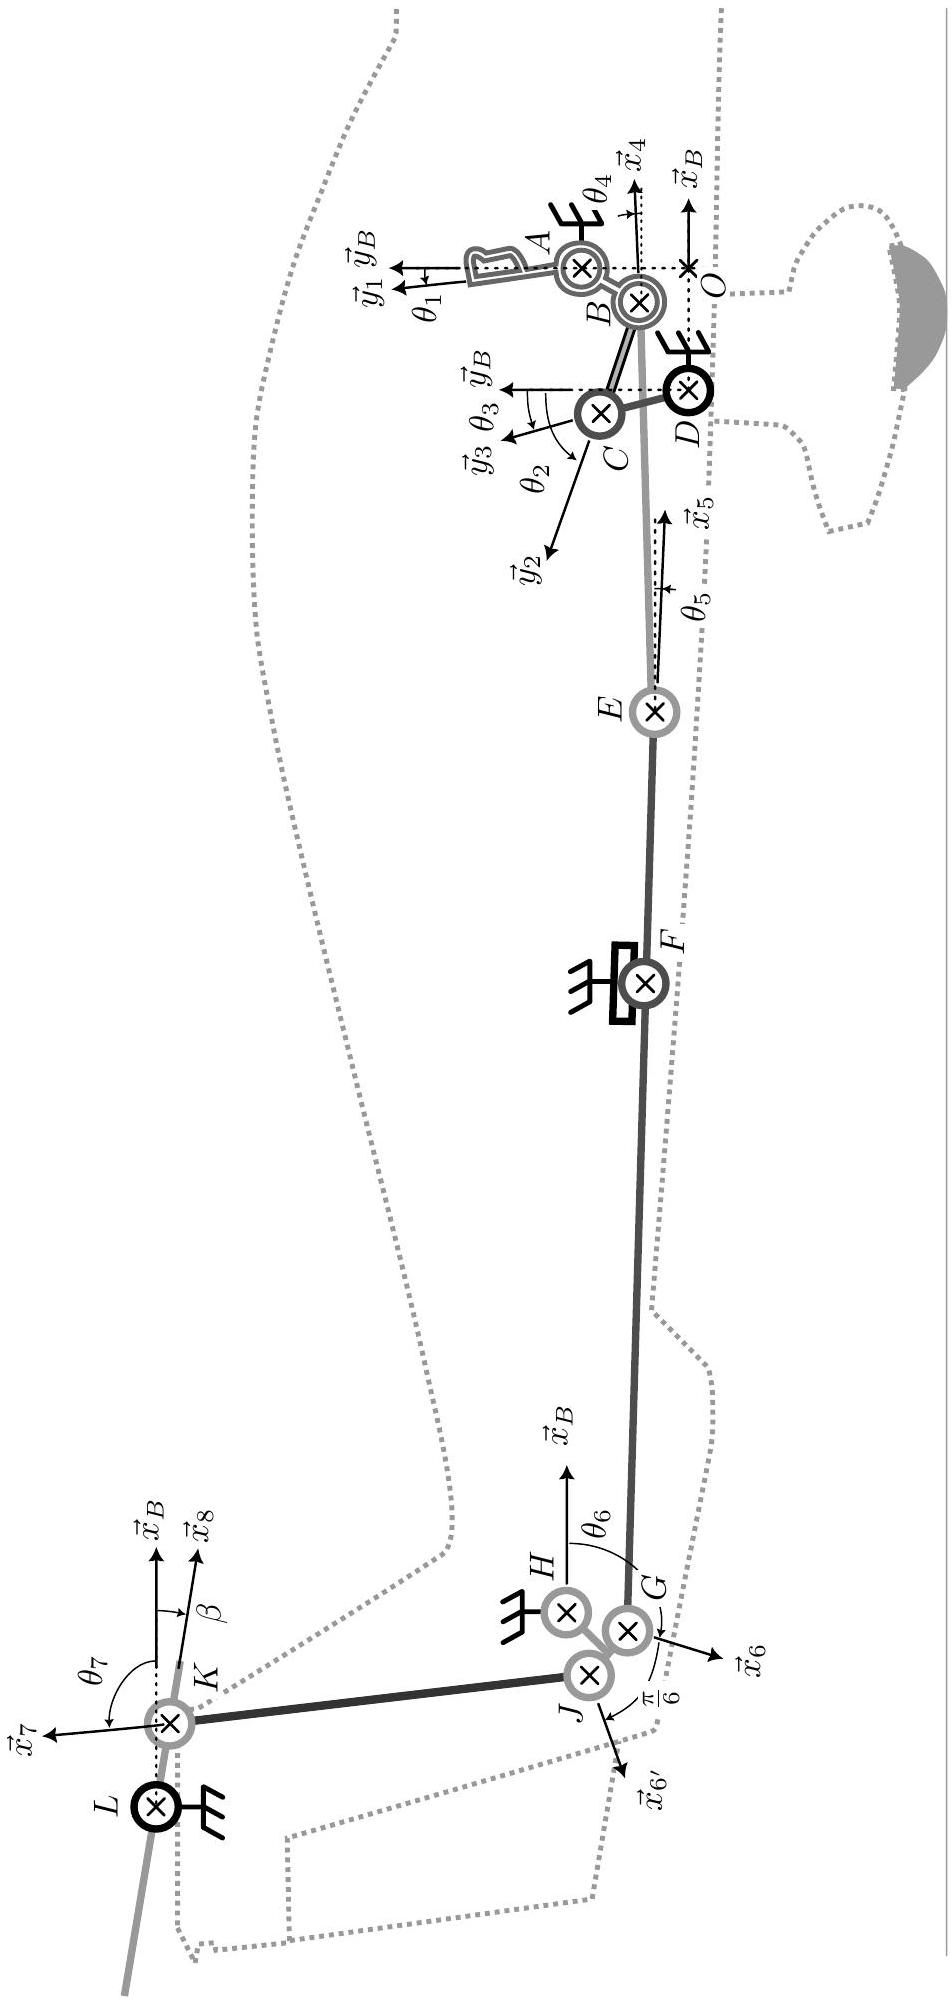
\includegraphics[max width=\textwidth, alt={}]{b437a5a5-8562-4c88-96c5-adc15de36bac-19_2002_951_450_145}
\end{center}

$$
\begin{gathered}
\overrightarrow{O A}=\left(0 ; Y_{A} ; 0\right)_{R_{B}} \quad \overrightarrow{O D}=\left(X_{D} ; 0 ; 0\right)_{R_{B}} \quad \overrightarrow{O F}=\left(X_{F} ; Y_{F} ; 0\right)_{R_{B}} \quad \overrightarrow{O H}=\left(X_{H} ; Y_{H} ; 0\right)_{R_{B}} \quad \overrightarrow{O L}=\left(X_{L} ; Y_{L} ; 0\right)_{R_{B}} \\
\|\overrightarrow{A B}\|=L_{1} \quad\|\overrightarrow{B C}\|=L_{2} \quad\|\overrightarrow{C D}\|=L_{3} \quad\|\overrightarrow{B E}\|=L_{4} \quad\|\overrightarrow{E G}\|=L_{5} \quad\|\overrightarrow{H G}\|=L_{6}=\|\overrightarrow{H J}\| \quad\|\overrightarrow{J K}\|=L_{7} \quad\|\overrightarrow{L K}\|=L_{8} \quad\|\overrightarrow{F E}\|=\lambda_{5}(t) \\
\left(\vec{x}_{B}, \vec{x}_{1}\right)=\left(\vec{y}_{B}, \vec{y}_{1}\right)=\theta_{1}(t) \quad\left(\vec{x}_{B}, \vec{x}_{2}\right)=\left(\vec{y}_{B}, \vec{y}_{2}\right)=\theta_{2}(t) \quad\left(\vec{x}_{B}, \vec{x}_{3}\right)=\left(\vec{y}_{B}, \vec{y}_{3}\right)=\theta_{3}(t) \quad\left(\vec{x}_{B}, \vec{x}_{4}\right)=\left(\vec{y}_{B}, \vec{y}_{4}\right)=\theta_{4}(t) \\
\left(\vec{x}_{B}, \vec{x}_{5}\right)=\left(\vec{y}_{B}, \vec{y}_{5}\right)=\theta_{5}(t) \quad\left(\vec{x}_{B}, \vec{x}_{6}\right)=\left(\vec{y}_{B}, \vec{y}_{6}\right)=\theta_{6}(t) \quad\left(\vec{x}_{B}, \vec{x}_{7}\right)=\left(\vec{y}_{B}, \vec{y}_{7}\right)=\theta_{7}(t) \quad\left(\vec{x}_{B}, \vec{x}_{8}\right)=\left(\vec{y}_{B}, \vec{y}_{8}\right)=\beta(t) \\
\left(\vec{x}_{6}, \vec{x}_{6^{\prime}}\right)=\left(\vec{y}_{6}, \vec{y}_{6^{\prime}}\right)=\frac{\pi}{6}
\end{gathered}
$$

Annexe D Réponses fréquentielle et temporelle de la boucle d'asservissement de la vitesse horizontale $V_{x}$

\begin{figure}[h]
\begin{center}
  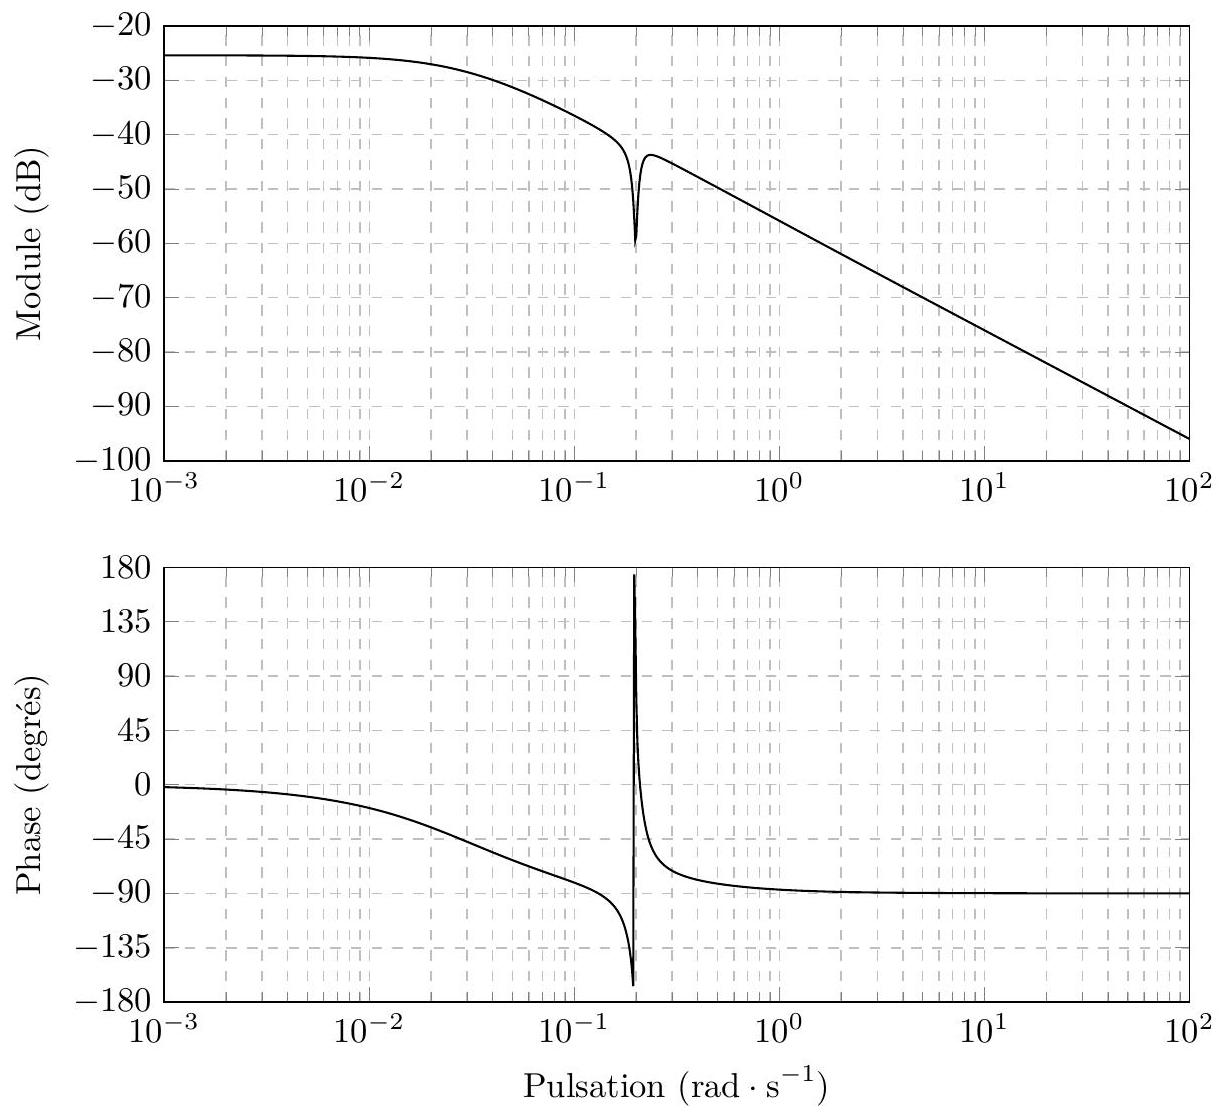
\includegraphics[alt={},max width=\textwidth]{b437a5a5-8562-4c88-96c5-adc15de36bac-20_1115_1224_302_413}
\captionsetup{labelformat=empty}
\caption{Figure 16 - Diagramme de Bode de $H_{1}(p)-B(p)$}
\end{center}
\end{figure}

\begin{figure}[h]
\begin{center}
  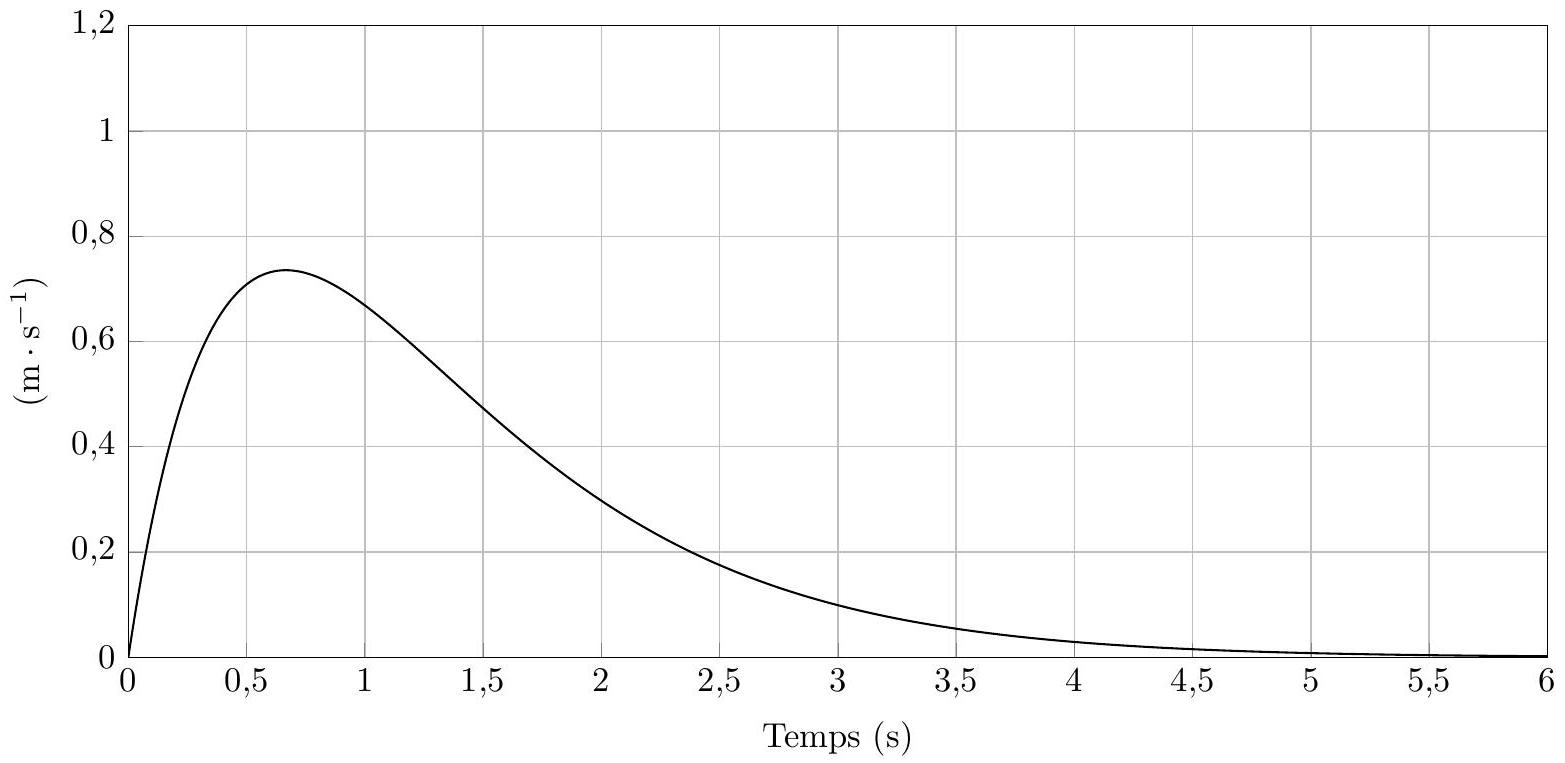
\includegraphics[alt={},max width=\textwidth]{b437a5a5-8562-4c88-96c5-adc15de36bac-20_763_1565_1576_244}
\captionsetup{labelformat=empty}
\caption{Figure 17 - Réponse indicielle de $T p \cdot X(p)$}
\end{center}
\end{figure}


\end{document}